\subsection{Restes de proies des ÉRES}

151 échantillons de restes de proies ont été collectés entre 2003 et 2013 (la période d'échantillonnage précoce) et 85 échantillons ont été collectés entre 2017 et 2023 (la période d'échantillonnage actuelle). Le nombre d'échantillons variait selon les strates spatiales et le mois (Figure \ref{fig:bar-diet}). Durant la période précoce, la majorité des échantillons ont été collectés du banc Swiftsure, de Nitinat et de Port Renfrew en juin, juillet et août, tandis que durant la période actuelle, Swiftsure et Nitinat en juillet et août étaient les strates les plus intensément échantillonnées. Bien que des relevés dédiés aux ÉRES aient eu lieu dans le centre du détroit Juan de Fuca et à Sooke/Victoria durant 2018 et 2019, aucun échantillon n'a été collecté. Les programmes de recherche de la NOAA ont collecté des échantillons dans ces strates plus récemment (B. Hanson, comm. pers.), mais ces échantillons n'ont pas été inclus ici. Aucun échantillon durant la période actuelle n'a été inclus du centre du détroit Juan de Fuca, de Sooke/Victoria, ou des strates des îles San Juan.

Nous avons tenté d'ajuster diverses structures de modèles aux données de restes de proies des ÉRES, mais il y avait trop peu d'observations pour capturer adéquatement la variabilité parmi les saisons, les strates spatiales, et les périodes d'échantillonnage précoce et actuelle. En conséquence, nous fournissons une description qualitative de la variabilité dans la composition des stocks. Le saumon quinnat Fraser été $4_1$ était le stock le plus communément observé, particulièrement en juillet et août. Durant la période d'échantillonnage précoce, les individus Fraser printemps $5_2$, et dans une moindre mesure été $5_2$, étaient communs dans les restes de proies durant juin et juillet. Le stock Columbia été/automne était régulièrement observé dans les strates du banc Swiftsure et de Port Renfrew, mais était rare plus à l'est. Le stock Puget Sound était observé tout au long de juin, juillet et août. Les stocks COIV-SOMN et COIV étaient relativement rarement observés.

\begin{figure}[H]
    \centering
    \pdftooltip{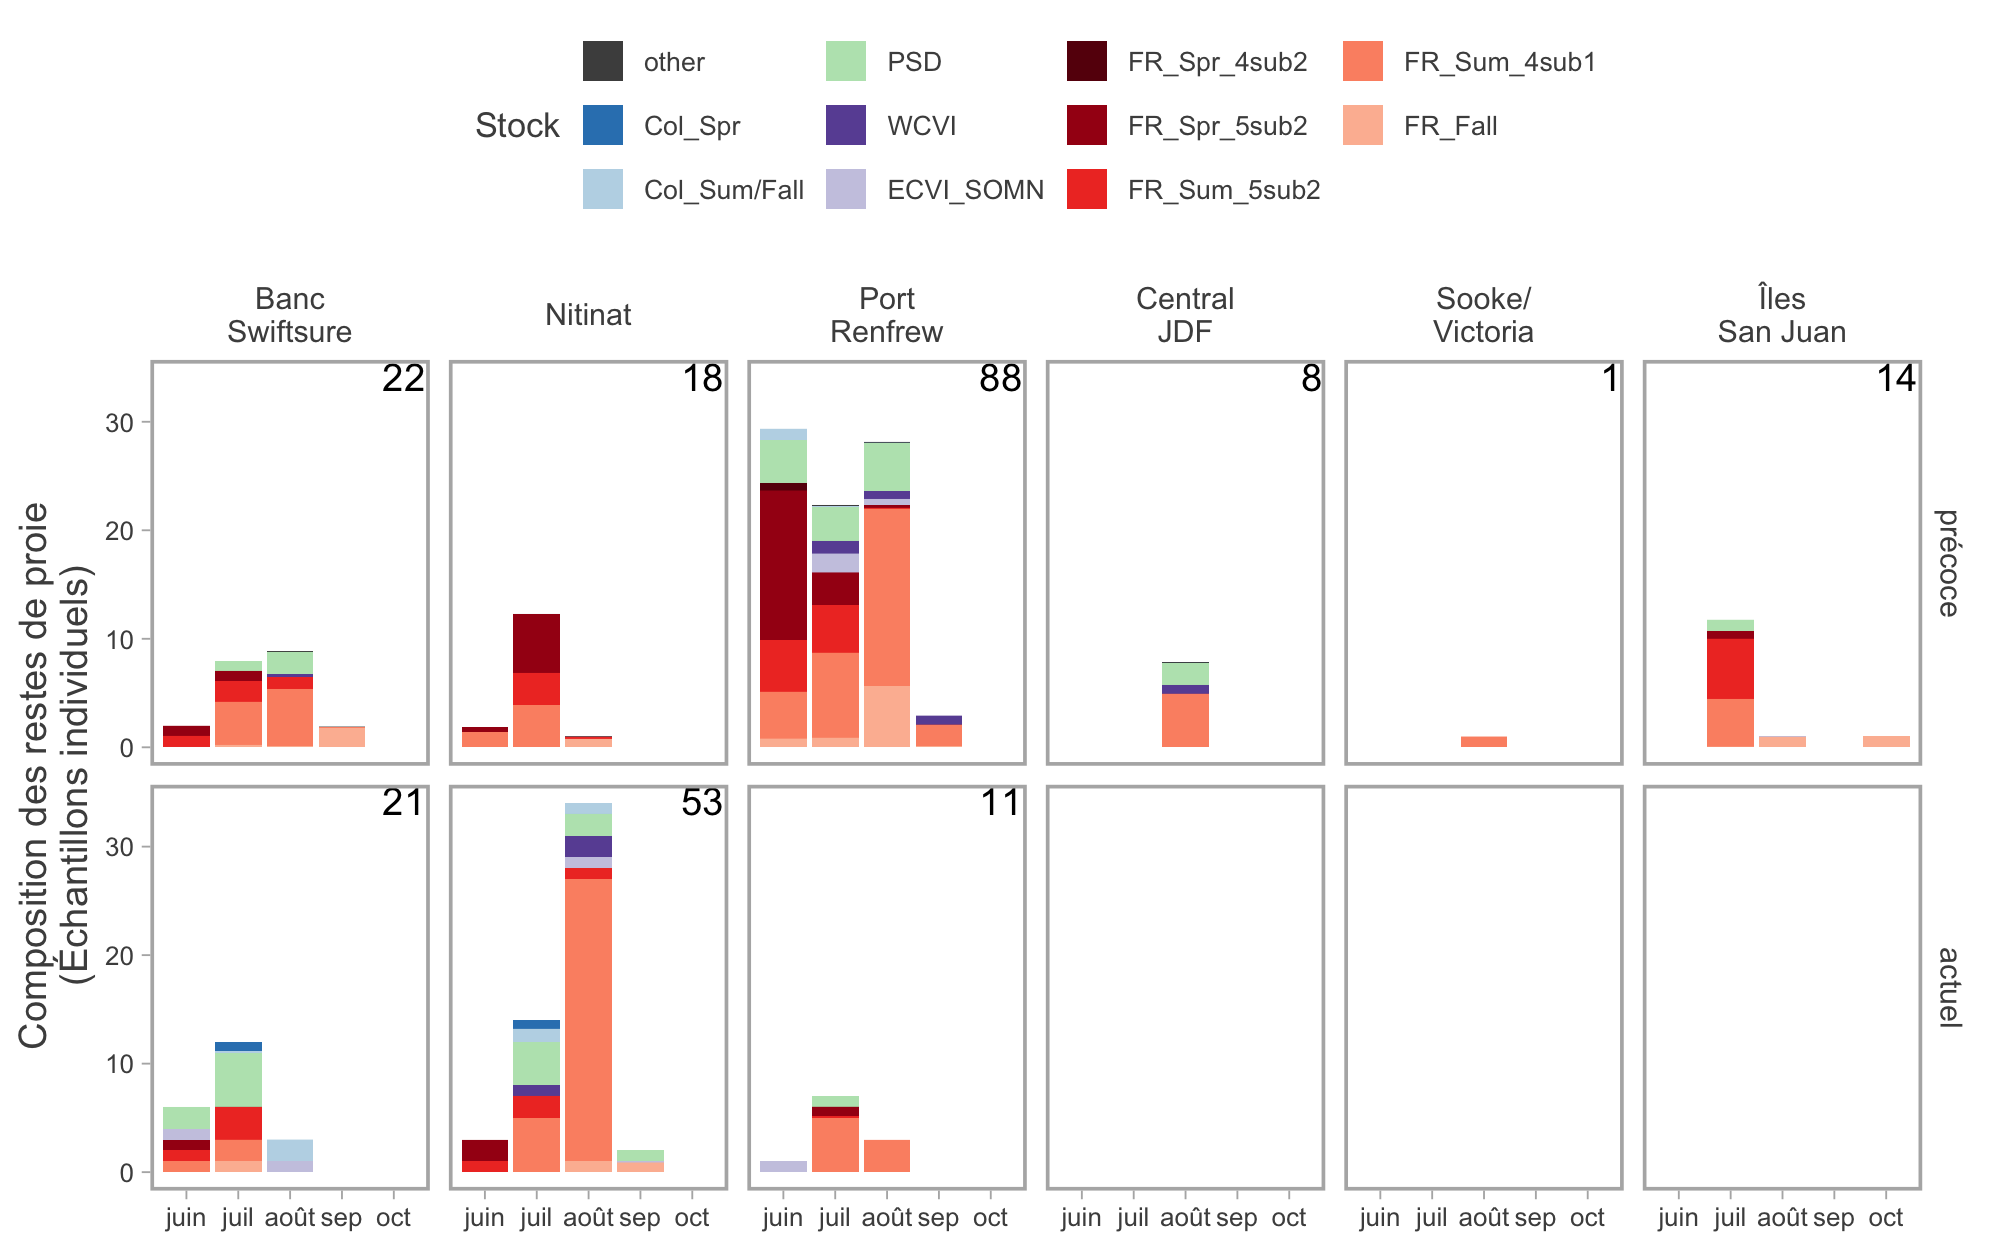
\includegraphics[width=5in]{figs/monthly_comp_bar.png}}{Figure \ref{fig:bar-diet}}
    \caption{Composition mensuelle des stocks de saumon quinnat dans les échantillons de restes de proies des ÉRES. Les strates (colonnes) correspondent aux domaines spatiaux de la Figure \ref{fig:sampling-map}. L'axe des Y représente le nombre d'échantillons collectés dans un mois-strate-période d'échantillonnage donnés. Les chiffres dans le coin supérieur droit de chaque panneau représentent la taille totale de l'échantillon dans chaque strate et période.}
    \label{fig:bar-diet}
\end{figure}

La probabilité que les échantillons d'origine d'écloserie puissent être identifiés de manière fiable dans les restes de proies était relativement faible car les taux de marquage TPB n'excédaient pas 80\% dans de nombreuses écloseries jusqu'à l'année de ponte 2015 ou plus tard (Figure \ref{fig:pbt-coverage}). Six échantillons de restes de proies appartenaient à des populations et des années de ponte avec un taux de marquage TPB supérieur à 80\%. De ceux-ci, trois ont été identifiés selon le stock basé sur le TPB--deux du ruisseau Robertson (COIV) et un de l'écloserie Chilliwack (Fraser automne) respectivement. Quatre autres échantillons de restes de proies ont été identifiés selon le stock basé sur le TPB, mais provenaient d'années population-ponte avec des taux de marquage inférieurs à 80\%--un individu chacun des écloseries Capilano (COIV-SOMN), Puntledge (COIV-SOMN), Big Qualicum (COIV-SOMN), et Chilliwack. Un échantillon de proie a été identifié avec une grande certitude (>99\%) comme provenant de la rivière Nitinat (une population COIV avec un taux PHOS >75\% durant plusieurs années) durant une année avec un faible taux TPB et a donc une probabilité raisonnablement élevée d'être d'origine d'écloserie. Aucun autre échantillon n'avait une assignation de stock qui suggérait une forte probabilité de provenir d'écloseries canadiennes basée sur des taux PHOS élevés (>75\%) durant les années récentes, bien que nous notions que ceci est une technique de classification incertaine.

La majorité des échantillons de restes de proies provenaient de saumons quinnat d'âge océanique-3. Les individus d'âge océanique-4 étaient relativement communs durant la période d'échantillonnage précoce, mais plus rarement observés durant la période actuelle. Peu de saumons quinnat d'âge océanique-2 et aucun d'âge océanique-1 n'ont été identifiés (Figure \ref{fig:bar-age-diet}). L'erreur de vieillissement, ainsi que la variation parmi les échantillons en âge, identité de stock, et date d'échantillonnage ont résulté en une variation additionnelle dans la taille corporelle estimée (Figure \ref{fig:bar-size-diet}). La probabilité que les poissons observés dans les régimes alimentaires étaient plus petits que $65$ cm était très faible à travers tous les mois et strates, tandis que les individus de $65-75$ cm étaient relativement rares. Durant la période précoce, la probabilité que les proies étaient dans la plus grande classe de taille $>85$ cm était relativement élevée, tandis que durant la période actuelle la classe de taille $75-85$ cm avait la plus grande probabilité. Cependant, les différences dans quand et où les échantillons ont été collectés empêchent un test quantitatif pour les changements dans la composition de la taille.

\begin{figure}[H]
    \centering
    \pdftooltip{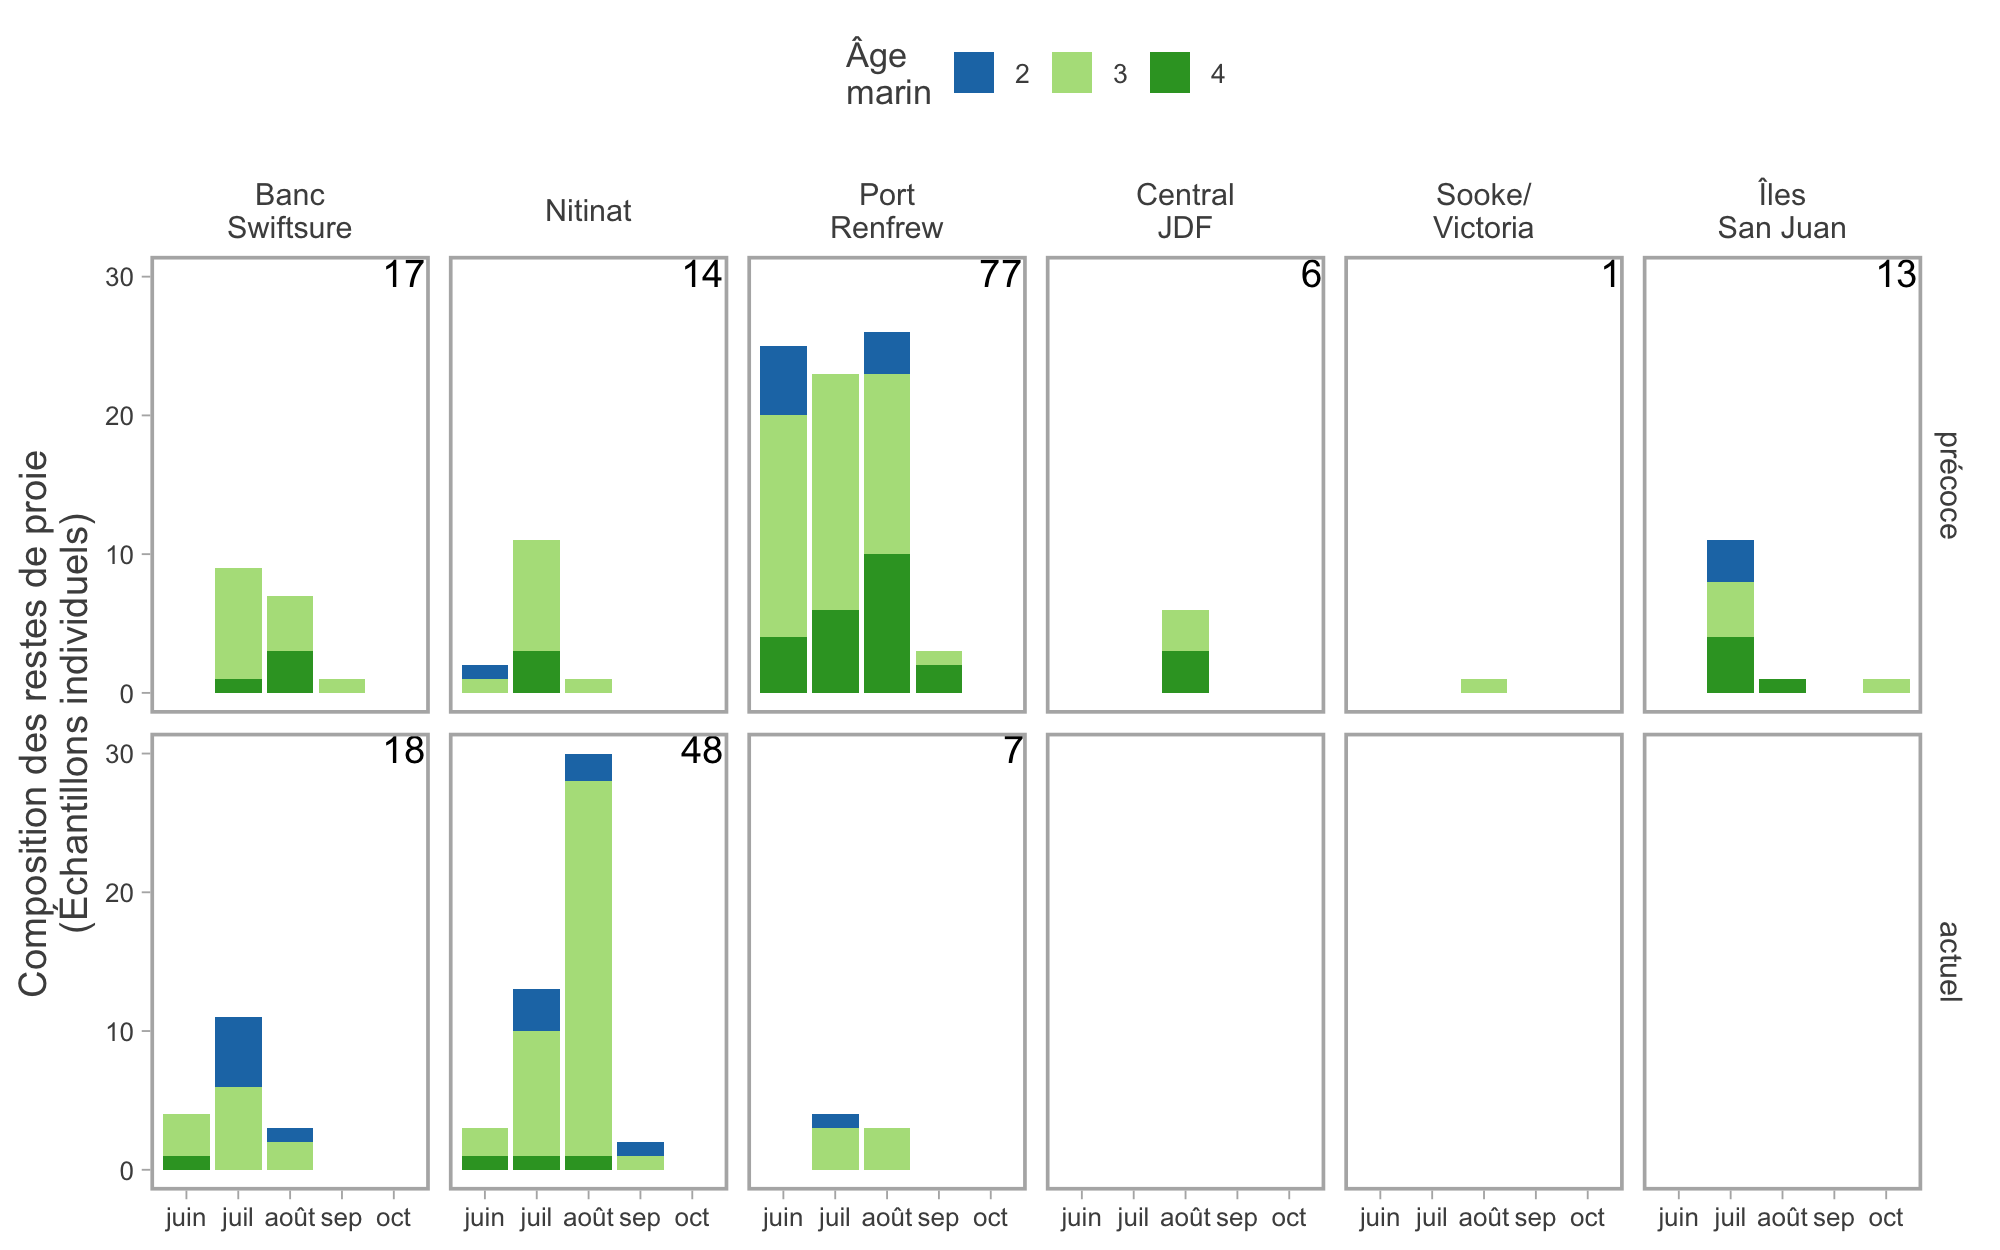
\includegraphics[width=5in]{figs/comp_bar_prey_age.png}}{Figure \ref{fig:bar-age-diet}}
    \caption{Composition mensuelle de l'âge marin du saumon quinnat dans les échantillons de restes de proies des ÉRES. Les données d'âge incorporent l'erreur d'observation associée aux estimations des annuli d'écailles. Les strates (colonnes) correspondent aux domaines spatiaux de la Figure \ref{fig:sampling-map}. L'axe des Y représente le nombre d'échantillons collectés dans un mois-strate-période d'échantillonnage donnés. Les chiffres dans le coin supérieur droit de chaque panneau représentent la taille totale de l'échantillon dans chaque strate et période.}
    \label{fig:bar-age-diet}
\end{figure}

\begin{figure}[H]
    \centering
    \pdftooltip{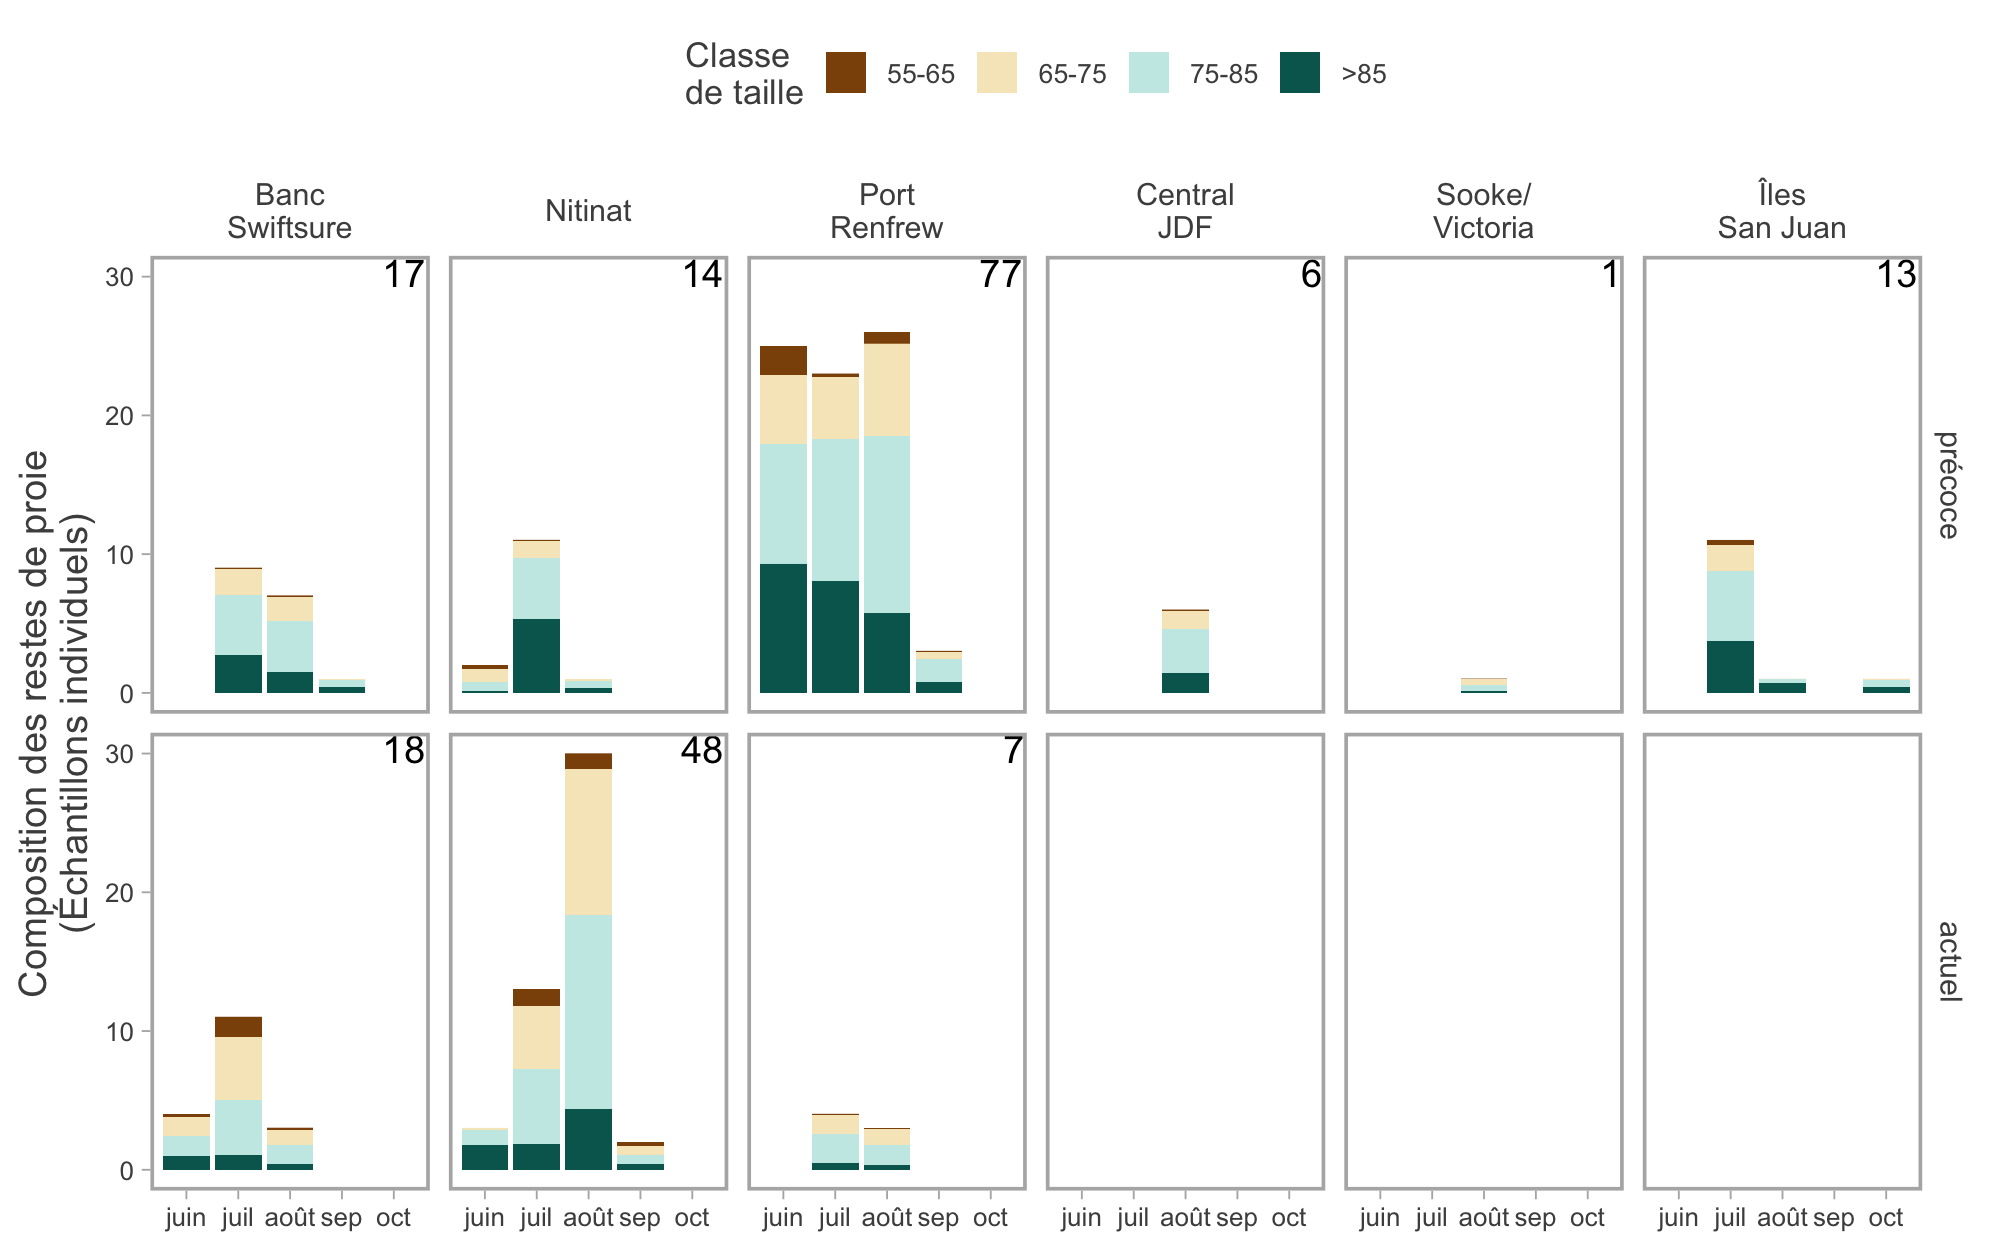
\includegraphics[width=5in]{figs/comp_bar_prey_size.png}}{Figure \ref{fig:bar-size-diet}}
    \caption{Composition mensuelle des classes de taille du saumon quinnat dans les échantillons de restes de proies des ÉRES basée sur les prédictions des modèles taille-selon-l'âge spécifiques aux saisons (Annexe \ref{size-at-age}). Les strates (colonnes) correspondent aux domaines spatiaux de la Figure \ref{fig:sampling-map}. L'axe des Y représente le nombre d'échantillons collectés dans un mois-strate-période d'échantillonnage donnés. Les chiffres dans le coin supérieur droit de chaque panneau représentent la taille totale de l'échantillon dans chaque strate et période.}
    \label{fig:bar-size-diet}
\end{figure}

\subsection{Pêches récréatives de saumon quinnat}

\subsubsection{Composition des stocks}

Il y avait 8 000 échantillons de saumon quinnat qui ont été collectés de saumons quinnat qui étaient (a) plus grands que 55 cm de longueur à la fourche, (b) capturés entre les zones à l'ouest du détroit Juan de Fuca et les îles Gulf du sud de 2014 à 2023, et (c) identifiés selon le stock. La majorité des échantillons de pêche récréative ont été collectés durant les mois d'été d'emplacements à l'intérieur des strates du banc Swiftsure, Port Renfrew, et Victoria/Sooke (Figures \ref{fig:bar-rec-summer}, \ref{fig:bar-rec-full}). Dans les strates où les échantillons de pêche étaient disponibles à travers toutes les saisons, la composition des stocks a transité d'être dominée par le stock Puget Sound entre novembre et mai vers un assemblage plus mixte durant l'été (Figure \ref{fig:bar-rec-full}).

\begin{figure}[H]
    \centering
    \pdftooltip{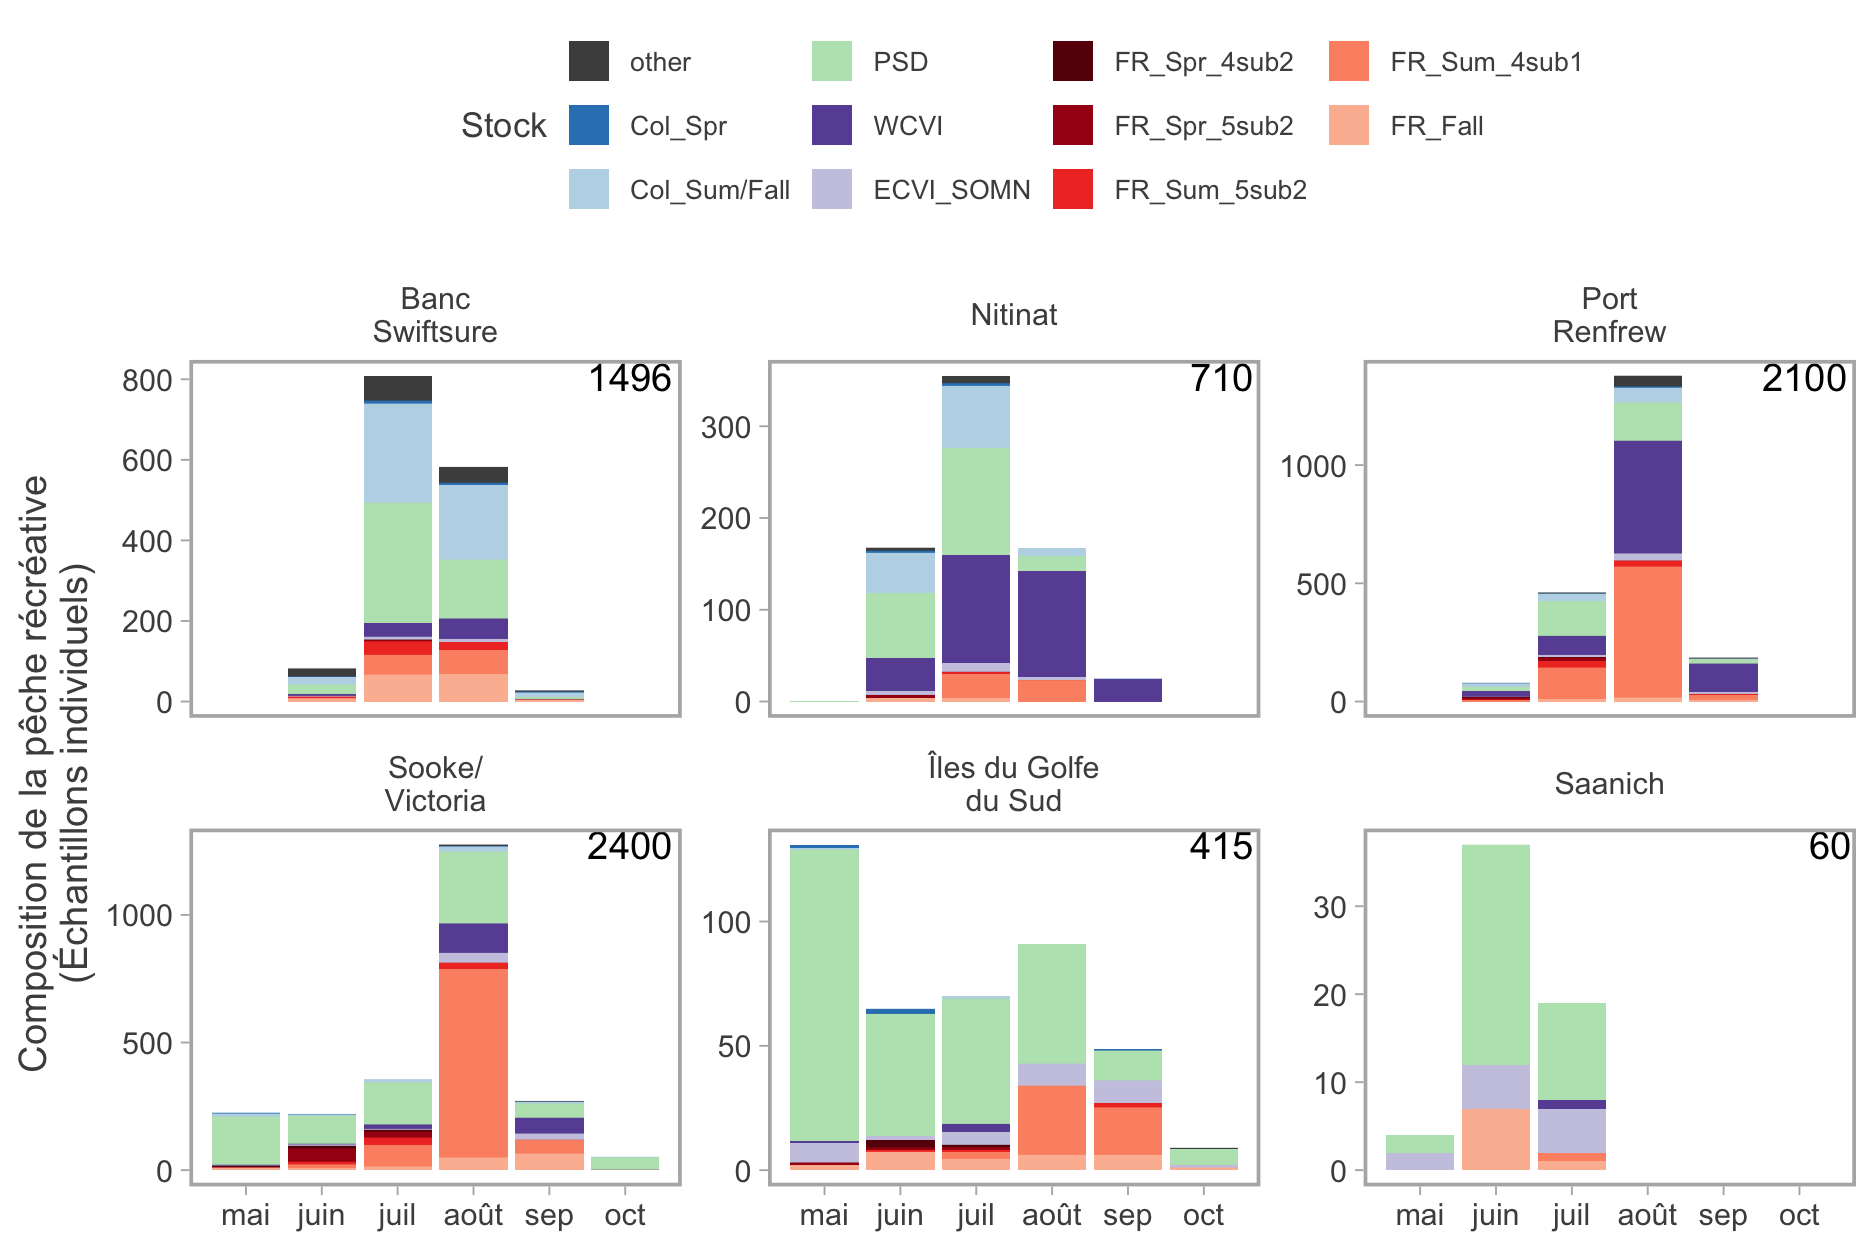
\includegraphics[width=5in]{figs/rec_monthly_comp_bar_summer.png}}{Figure \ref{fig:bar-rec-summer}}
    \caption{Composition mensuelle (mai-octobre) des stocks d'échantillons de pêche récréative de saumon quinnat. Les strates (panneaux) correspondent aux domaines spatiaux de la Figure \ref{fig:sampling-map}. L'axe des Y représente le nombre d'échantillons collectés dans un mois et une strate spatiale donnés. Les chiffres dans le coin supérieur droit de chaque panneau représentent la taille totale de l'échantillon dans chaque strate.}
    \label{fig:bar-rec-summer}
\end{figure}

La moyenne et la variance de la longueur à la fourche différaient parmi les stocks (Figure \ref{fig:density-fl}). Les poissons COIV, Fraser printemps $5_2$, été $5_2$, et été $4_1$ étaient typiquement plus grands (longueurs médianes entre 75 et 80 cm), tandis que les stocks Puget Sound et COIV-SOMN étaient relativement plus petits (longueurs médianes inférieures à 70 cm). Le stock Fraser rivière été $4_1$ avait une distribution de taille plus homogène (CV=0,09) que les stocks Puget Sound, Columbia rivière printemps, Fraser rivière automne, et COIV-SOMN (CV=0,12-0,13).

\begin{figure}[H]
    \centering
    \pdftooltip{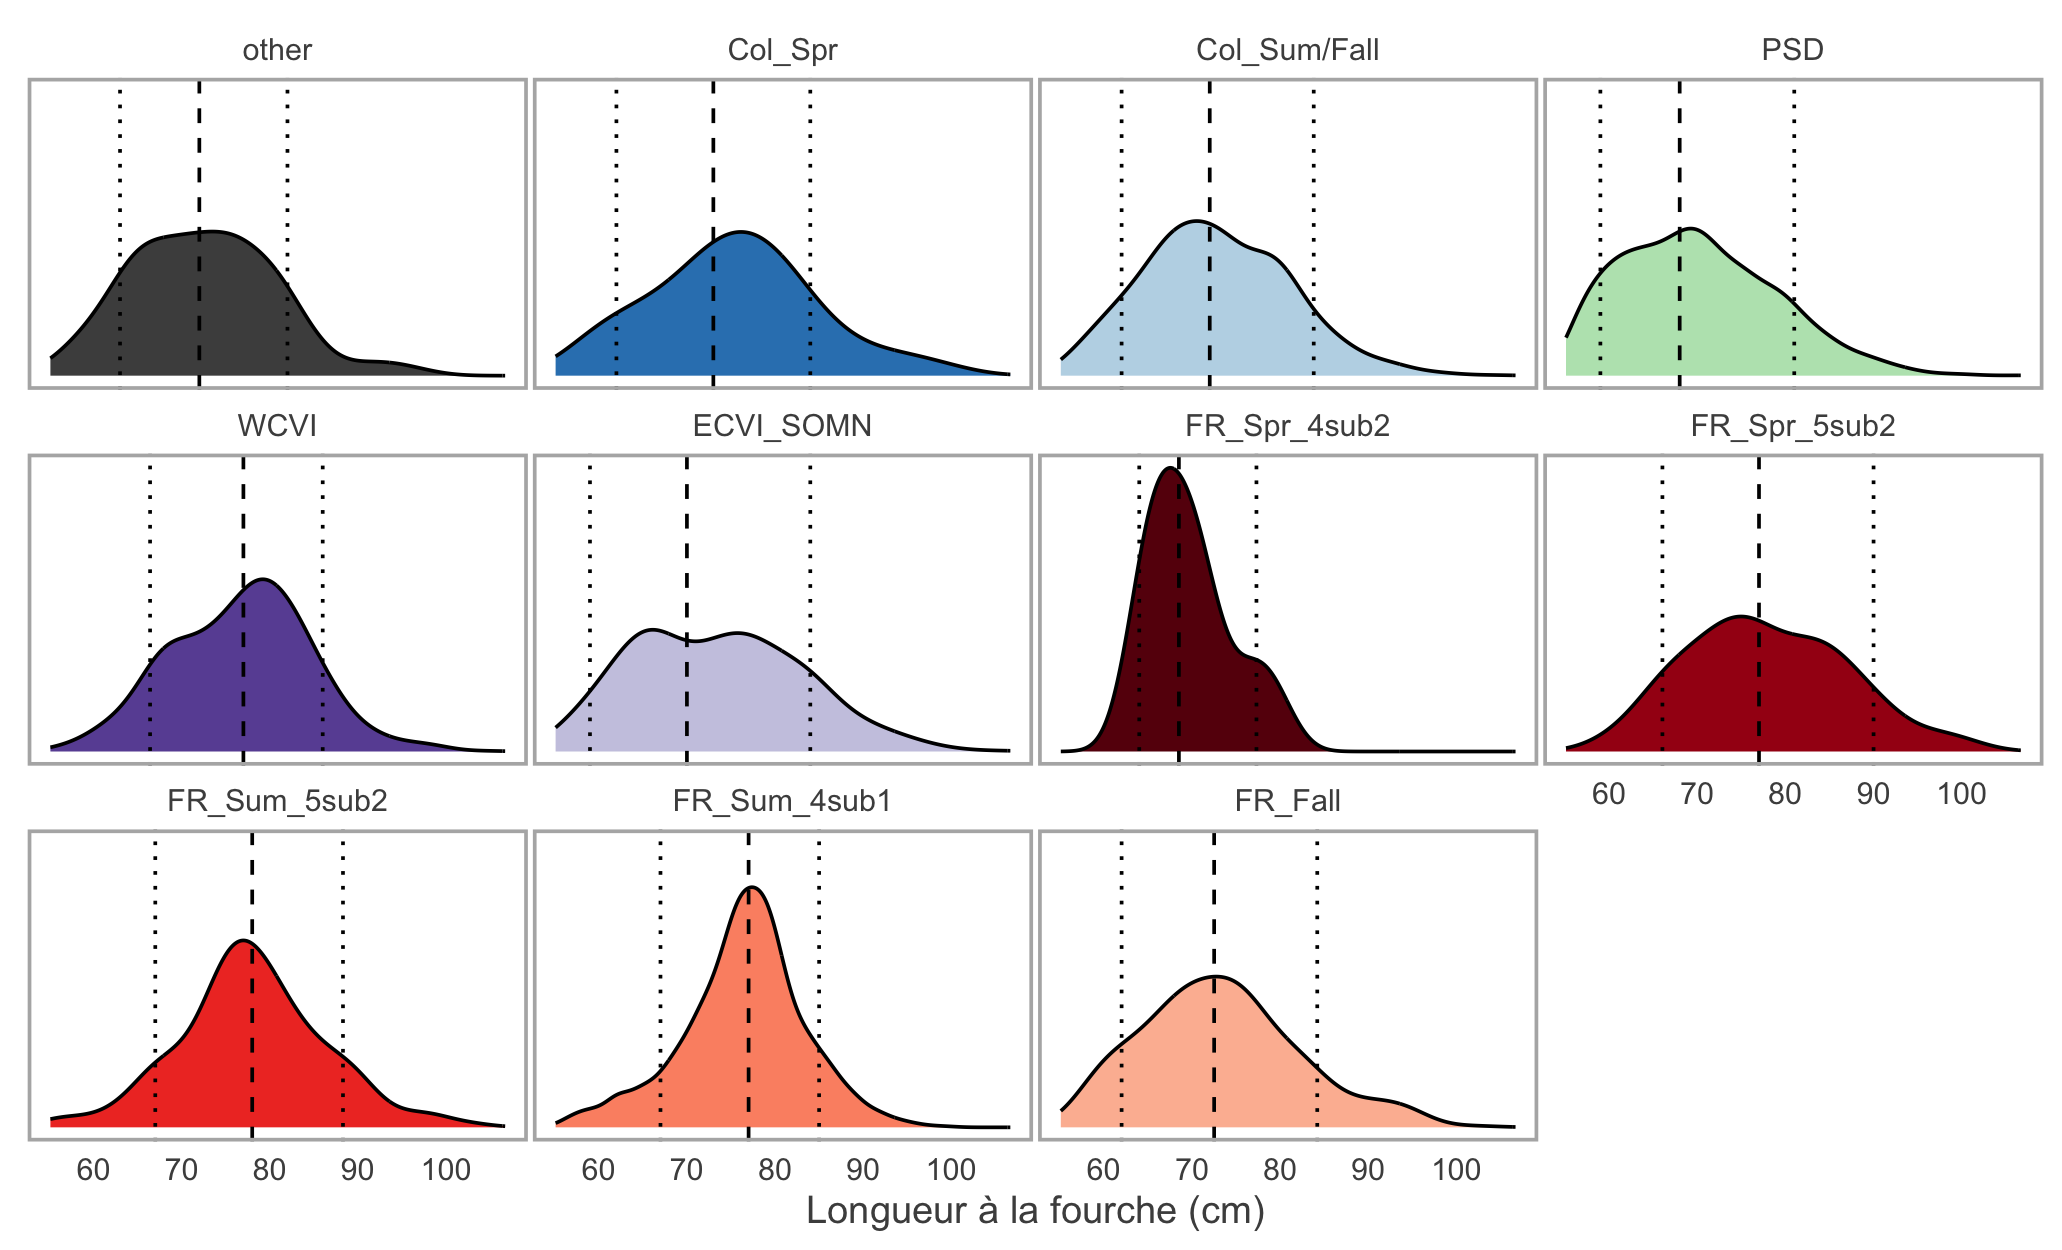
\includegraphics[width=5in]{figs/size_density.png}}{Figure \ref{fig:density-fl}}
    \caption{Estimations de densité par noyau de la longueur à la fourche (mm) spécifique aux stocks observée d'échantillons de pêche récréative de saumon quinnat (collectés entre mai-octobre). Les lignes verticales représentent les médianes spécifiques aux stocks (pointillées) et les intervalles du 80e percentile (ponctuées). Notez que les échantillons plus petits que 55 cm sont exclus. Notez que l'échelle de l'axe des y diffère parmi les strates.}
    \label{fig:density-fl}
\end{figure}

Notre modèle statistique a capturé la variabilité saisonnière, spatiale, et interannuelle dans l'abondance relative des stocks de saumon quinnat, tout en tenant compte de l'effort d'échantillonnage inégal. Les stocks de saumon quinnat différaient non seulement dans l'abondance relative moyenne, mais aussi les tendances saisonnières dans l'abondance relative. L'abondance relative des stocks juvéniles Fraser (c.-à-d., printemps $4_2$, printemps $5_2$, et été $5_2$) a décliné au cours de l'été, tandis que l'abondance Puget Sound a décliné durant l'été puis s'est rétablie durant septembre (Figure \ref{fig:season-pred-rec}). Les stocks Fraser été $4_1$ et COIV ont tous deux atteint l'abondance maximale à la fin de l'été, mais avec des pics à plusieurs semaines d'intervalle, tandis que le stock Fraser automne a atteint un pic à la fin septembre (Figure \ref{fig:season-pred-rec}).

\begin{figure}[H]
    \centering
    \pdftooltip{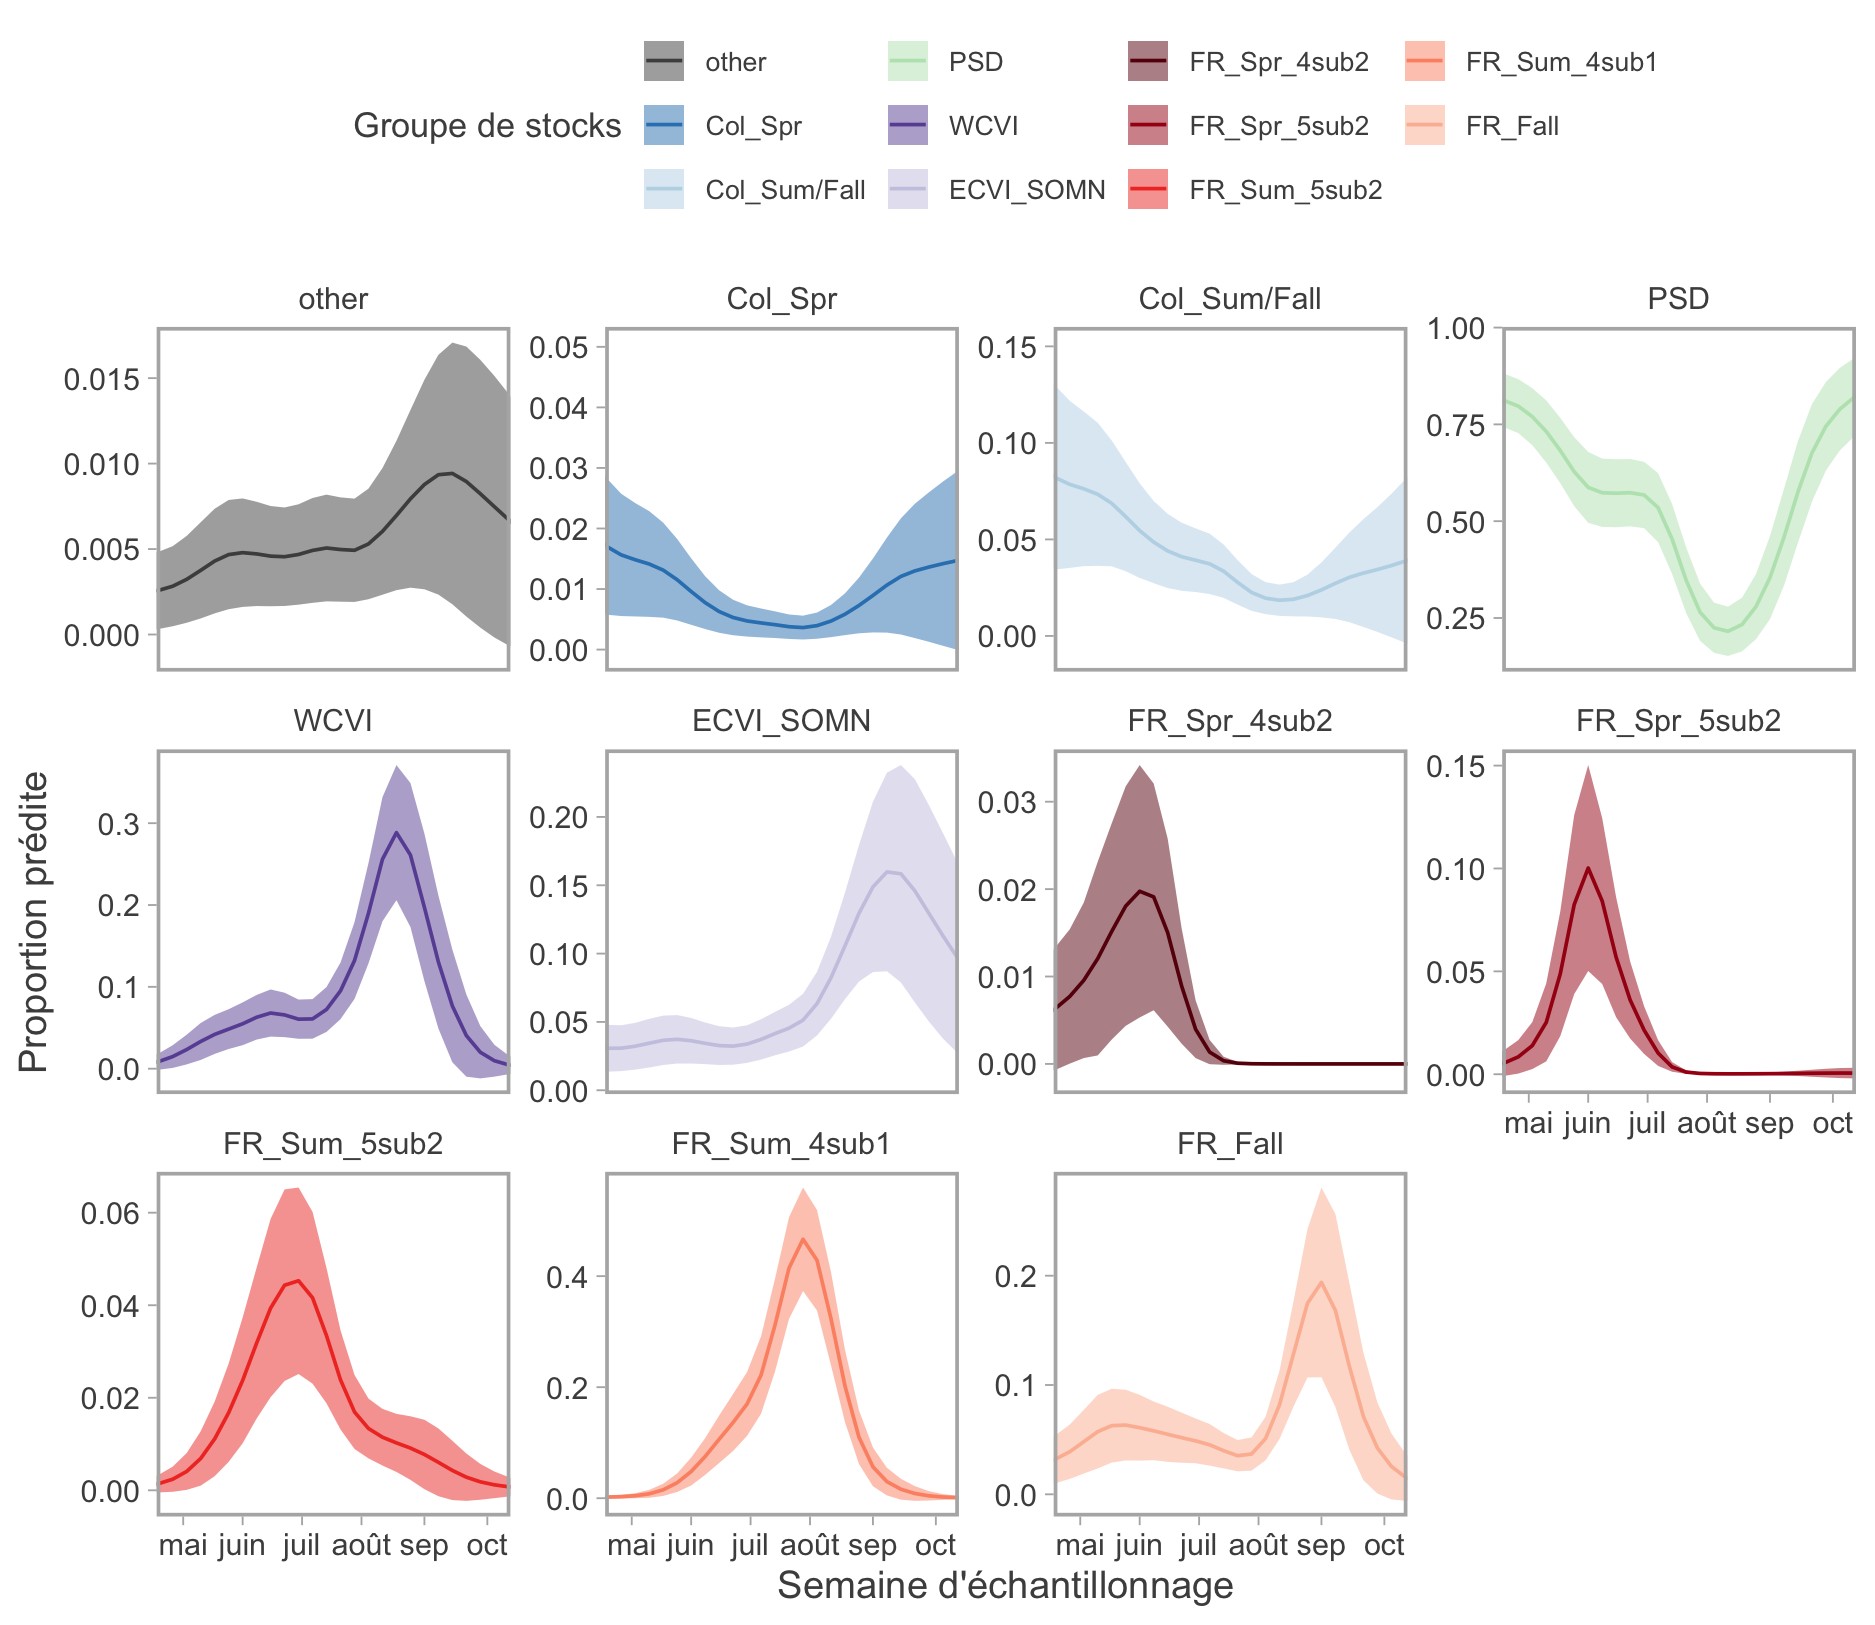
\includegraphics[width=5in]{figs/season_preds_chinook.png}}{Figure \ref{fig:season-pred-rec}}
    \caption{Composition saisonnière moyenne prédite des stocks, basée sur un modèle ajusté aux échantillons de pêche récréative, de mai à octobre. Le ruban représente l'intervalle de confiance à 95\% de la prédiction moyenne. Les prédictions représentent les effets conditionnels, excluant les covariables spatiales (c.-à-d., représentent l'effet saisonnier moyen à l'intérieur de la zone d'étude). Notez que l'échelle de l'axe des y diffère parmi les stocks.}
    \label{fig:season-pred-rec}
\end{figure}

Les stocks montraient aussi des distributions spatiales uniques. Les stocks 'Autre', Columbia printemps, Columbia été/automne, et Fraser automne étaient à leur abondance la plus élevée près de l'embouchure du détroit Juan de Fuca et du banc Swiftsure, tandis que le stock Puget Sound montrait le patron opposé (Figure \ref{fig:spatial-pred-scaled}). Le stock COIV était concentré près des côtes, particulièrement près du lac Nitinat, tandis que les stocks Fraser printemps $4_2$, printemps $5_2$, été $5_2$, et été $4_1$ étaient les plus abondants au milieu du détroit Juan de Fuca (Figure \ref{fig:spatial-pred-scaled}). Les prédictions non mises à l'échelle soulignent que la composition des stocks, en moyennant parmi les mois de mai à octobre, variait spatialement. Généralement Columbia été/automne et Puget Sound étaient les stocks dominants---le premier sur le banc Swiftsure et le dernier dans le sud du détroit de Georgie (Figure \ref{fig:spatial-pred}). Le stock COIV était dominant dans les emplacements côtiers près du lac Nitinat, tandis que le détroit Juan de Fuca avait une composition de stocks plus équilibrée due à l'abondance relativement élevée du stock Fraser été $4_1$ (Figure \ref{fig:spatial-pred}).

\begin{figure}[H]
    \centering
    \pdftooltip{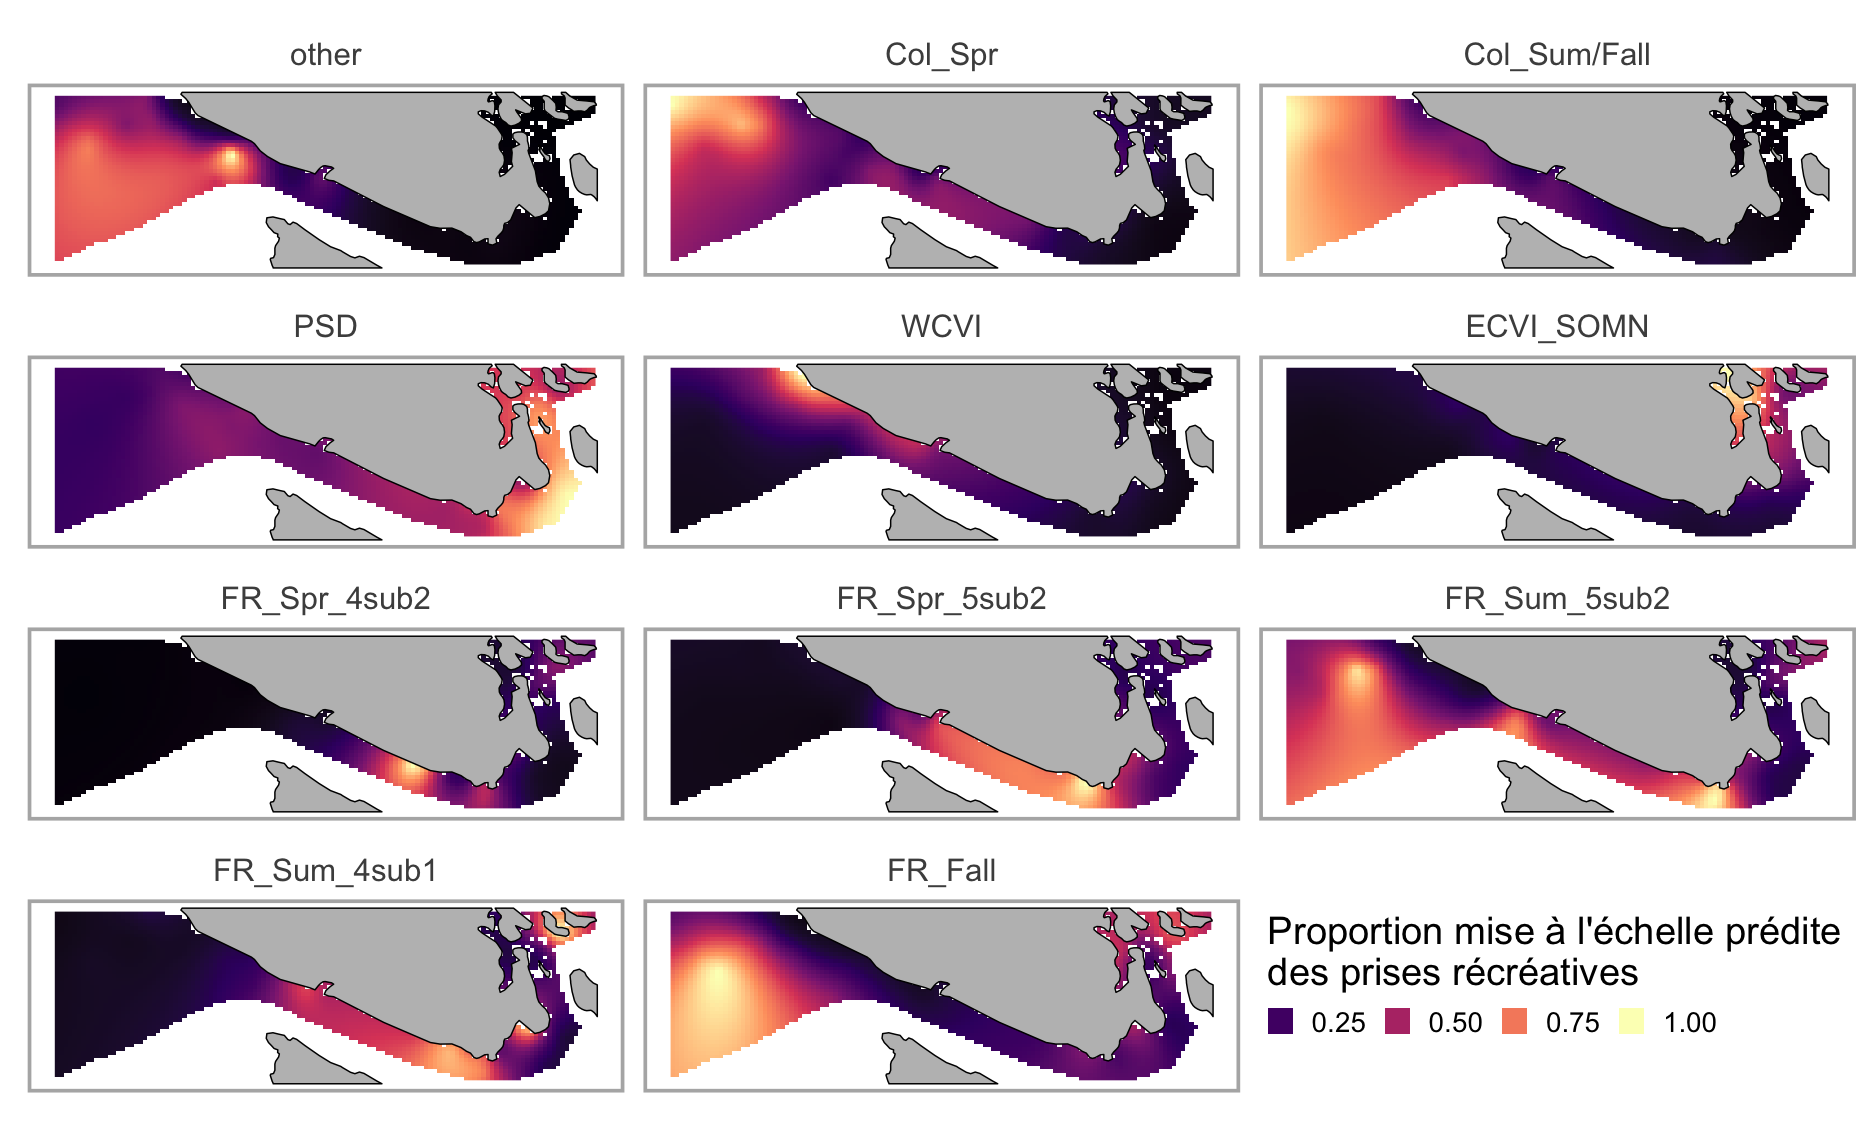
\includegraphics[width=5in]{figs/spatial_preds_scaled.png}}{Figure \ref{fig:spatial-pred-scaled}}
    \caption{Variation spatiale dans la composition moyenne prédite des stocks mise à l'échelle à travers la portion canadienne du détroit Juan de Fuca et le sud du détroit de Georgie basée sur les échantillons de pêche récréative. Les prédictions sont des moyennes spécifiques aux stocks pour mai à octobre et ont été mises à l'échelle relativement à la prédiction maximale à l'intérieur d'un stock pour souligner les différences spécifiques aux stocks. Une valeur de un (zéro) indique l'emplacement où un stock était à son abondance prédite maximale (minimale).}
    \label{fig:spatial-pred-scaled}
\end{figure}

\begin{figure}[H]
    \centering
    \pdftooltip{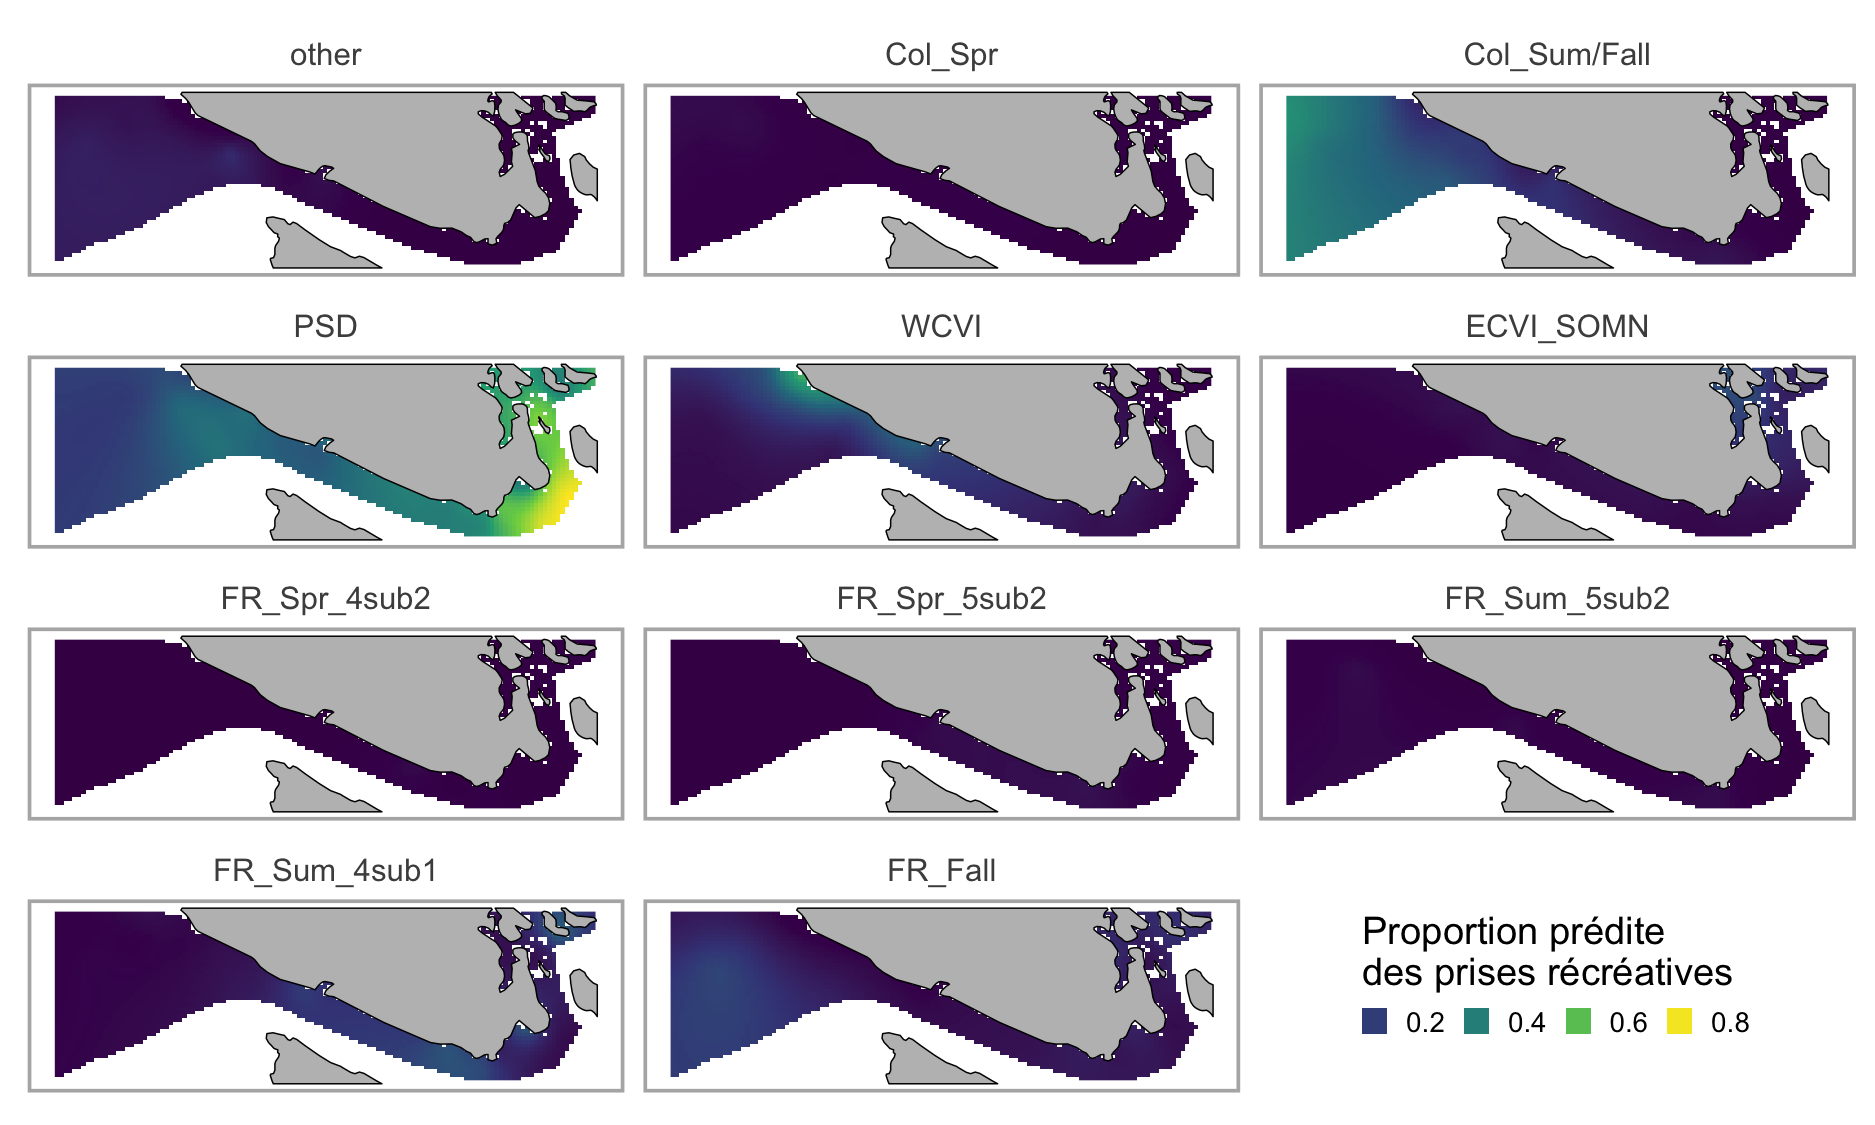
\includegraphics[width=5in]{figs/spatial_preds.png}}{Figure \ref{fig:spatial-pred}}
    \caption{Variation spatiale dans la composition moyenne prédite des stocks à travers la portion canadienne du détroit Juan de Fuca et le sud du détroit de Georgie basée sur les échantillons de pêche récréative. Les prédictions sont des moyennes spécifiques aux stocks pour mai à octobre. Une valeur de un (zéro) indique qu'un stock représentait 100\% (0\%) de l'échantillon moyen prédit.}
    \label{fig:spatial-pred}
\end{figure>

Les prédictions saisonnières de la composition moyenne des stocks pour des strates spécifiques soulignent simultanément la variabilité spatiale et temporelle dans l'abondance relative de différents stocks (Figure \ref{fig:stacked-rec}). Près du banc Swiftsure, les stocks Puget Sound et Columbia été/automne constituaient plus de 90\% de la capture en juin, mais les stocks Fraser été $4_1$ et COIV constituaient des composantes significatives de la capture au fur et à mesure que l'été progressait. Nitinat montrait un patron similaire, sauf avec une contribution beaucoup plus grande d'individus COIV, particulièrement en août et septembre quand ce stock constituait plus de 50\% de la capture. Les strates Port Renfrew et Sooke/Victoria montraient la plus grande contribution de poissons appartenant aux stocks de la rivière Fraser. Les poissons en route vers Fraser constituaient approximativement 50\% de la capture en août, prédominamment le stock été $4_1$, mais les stocks avec une chronologie de montaison plus précoce étaient quelque peu communs en juin. Les strates Port Renfrew et Sooke/Victoria différaient principalement dans la proportion des stocks Puget Sound et COIV. Les strates des îles Gulf du sud montraient une composition de stocks similaire à Sooke/Victoria, mais incluaient plus d'individus COIV/SOMN.

\begin{figure}[H]
    \centering
    \pdftooltip{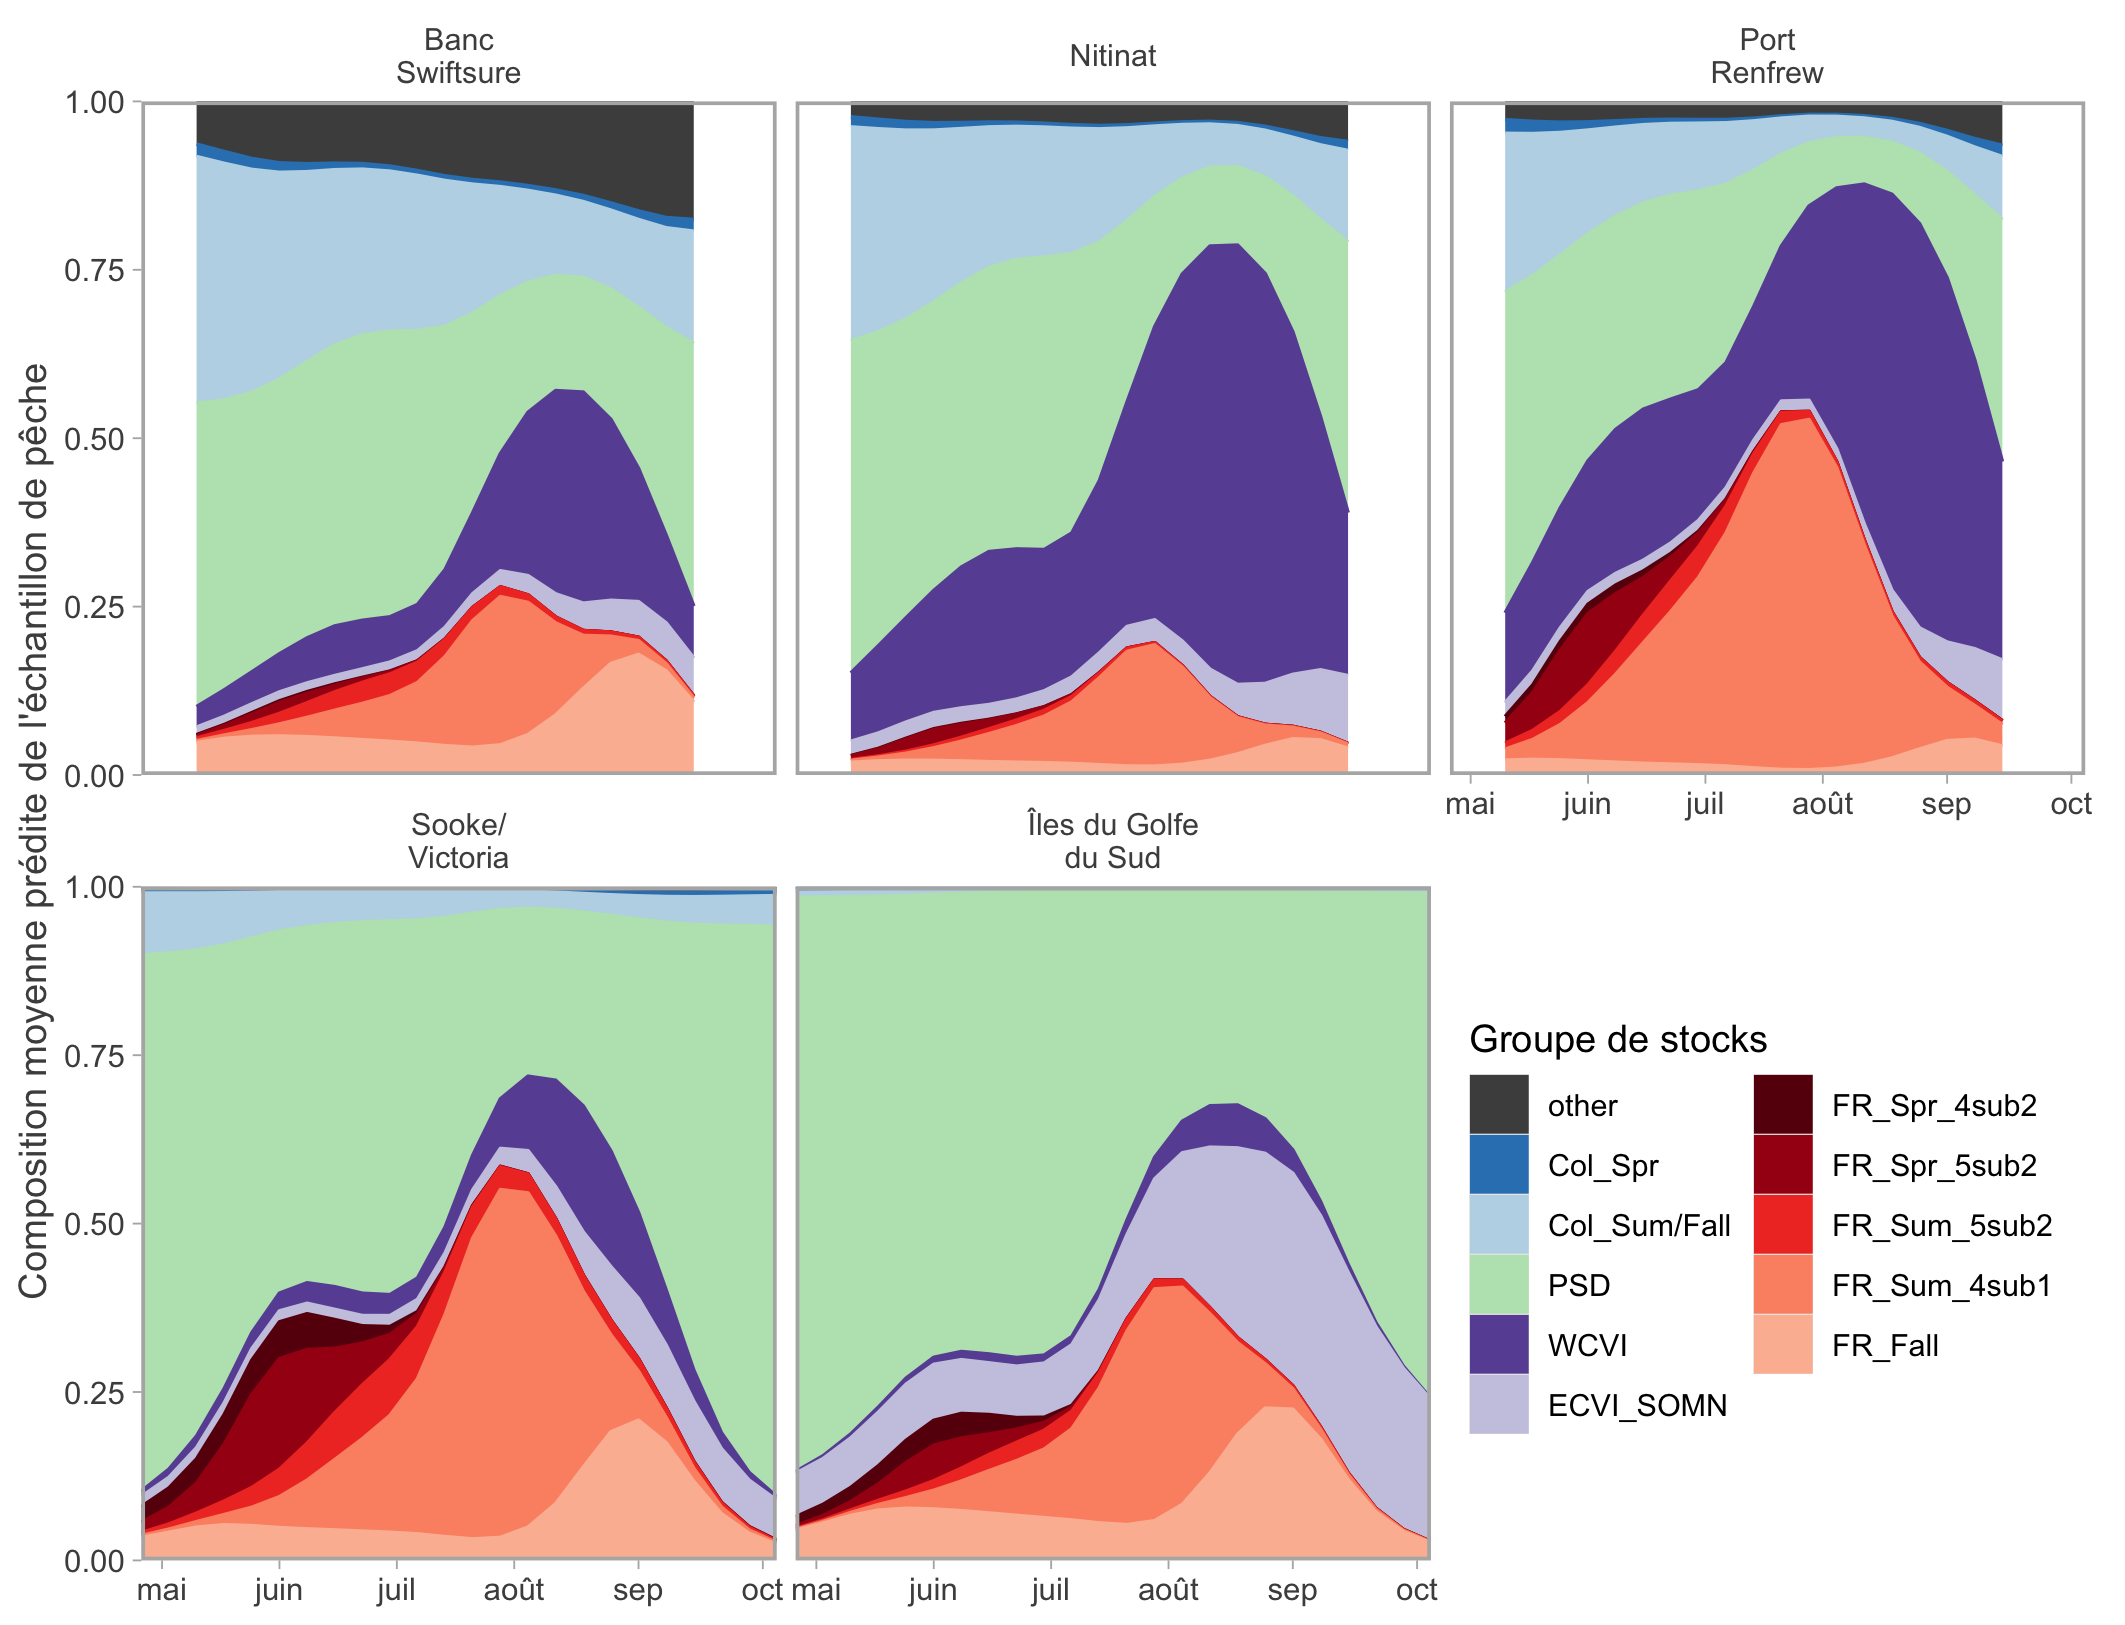
\includegraphics[width=5in]{figs/smooth_preds_chinook_stacked.png}}{Figure \ref{fig:stacked-rec}}
    \caption{Composition saisonnière moyenne prédite des stocks durant les mois d'été parmi cinq strates spatiales basée sur les échantillons de pêche récréative. Les prédictions ont été estimées en utilisant les emplacements (représentés par un « x ») à l'intérieur de chaque domaine spatial de la Figure \ref{fig:sampling-map} et excluent la variabilité interannuelle. Saanich non montré en raison de données limitées en juillet et août, ainsi que son emplacement à l'extérieur de l'habitat essentiel des ÉRES.}
    \label{fig:stacked-rec}
\end{figure}

La variabilité interannuelle dans l'abondance relative différait parmi les stocks et les emplacements spatiaux. Les stocks Columbia rivière printemps, Puget Sound, et COIV étaient relativement stables comparés aux stocks restants (Figure \ref{fig:smooth-pred-rec-year}). Par exemple, la proportion moyenne prédite de l'échantillon appartenant au Fraser rivière été $5_2$ à Sooke/Victoria en juillet variait de 4,6\% à 17,7\% parmi les années.

Les résidus du modèle ajusté étaient appropriément distribués (Figure \ref{fig:qqplot-stock}) et les vérifications prédictives postérieures ont confirmé que la composition moyenne simulée des stocks, tenant compte de la variance résiduelle, était généralement similaire à la composition observée des stocks (Figures \ref{fig:posterior-stock1}, \ref{fig:posterior-stock2}, \ref{fig:posterior-stock3}). Cependant la nature hiérarchique des modèles spatio-temporels, qui était nécessaire pour générer des prédictions pour un nombre relativement grand de stocks, a résulté en un rétrécissement qui tirait les observations individuelles vers la moyenne globale. En conséquence, les observations des strates avec relativement peu d'échantillons, comme Saanich, et les combinaisons stock-strates avec des patrons saisonniers fortement non-linéaires (p. ex., COIV à Nitinat) déviaient le plus fortement des prédictions du modèle.

\subsubsection{Composition de la taille}

Nous avons évalué la composition de la taille en utilisant les données de 10 651 saumons quinnat, plus grands que 55 cm de longueur à la fourche. Bien que la taille totale de l'échantillon pour l'analyse de composition de la taille était plus grande, plusieurs échantillons étaient partagés avec l'ensemble de données de composition des stocks décrit précédemment, résultant en une distribution saisonnière et spatiale similaire d'échantillons. Les individus plus petits que 75 cm étaient relativement communs dans les strates du banc Swiftsure, des îles Gulf du sud, et de Saanich, tandis que les classes de taille plus grandes étaient les plus abondantes à Nitinat et Port Renfrew (Figure \ref{fig:bar-rec-summer-size}). Dans les strates où les échantillons étaient disponibles à travers toutes les saisons, les poissons plus grands que 75 cm étaient largement absents avant mai et après septembre (Figure \ref{fig:bar-rec-full-size}).

\begin{figure}[H]
    \centering
    \pdftooltip{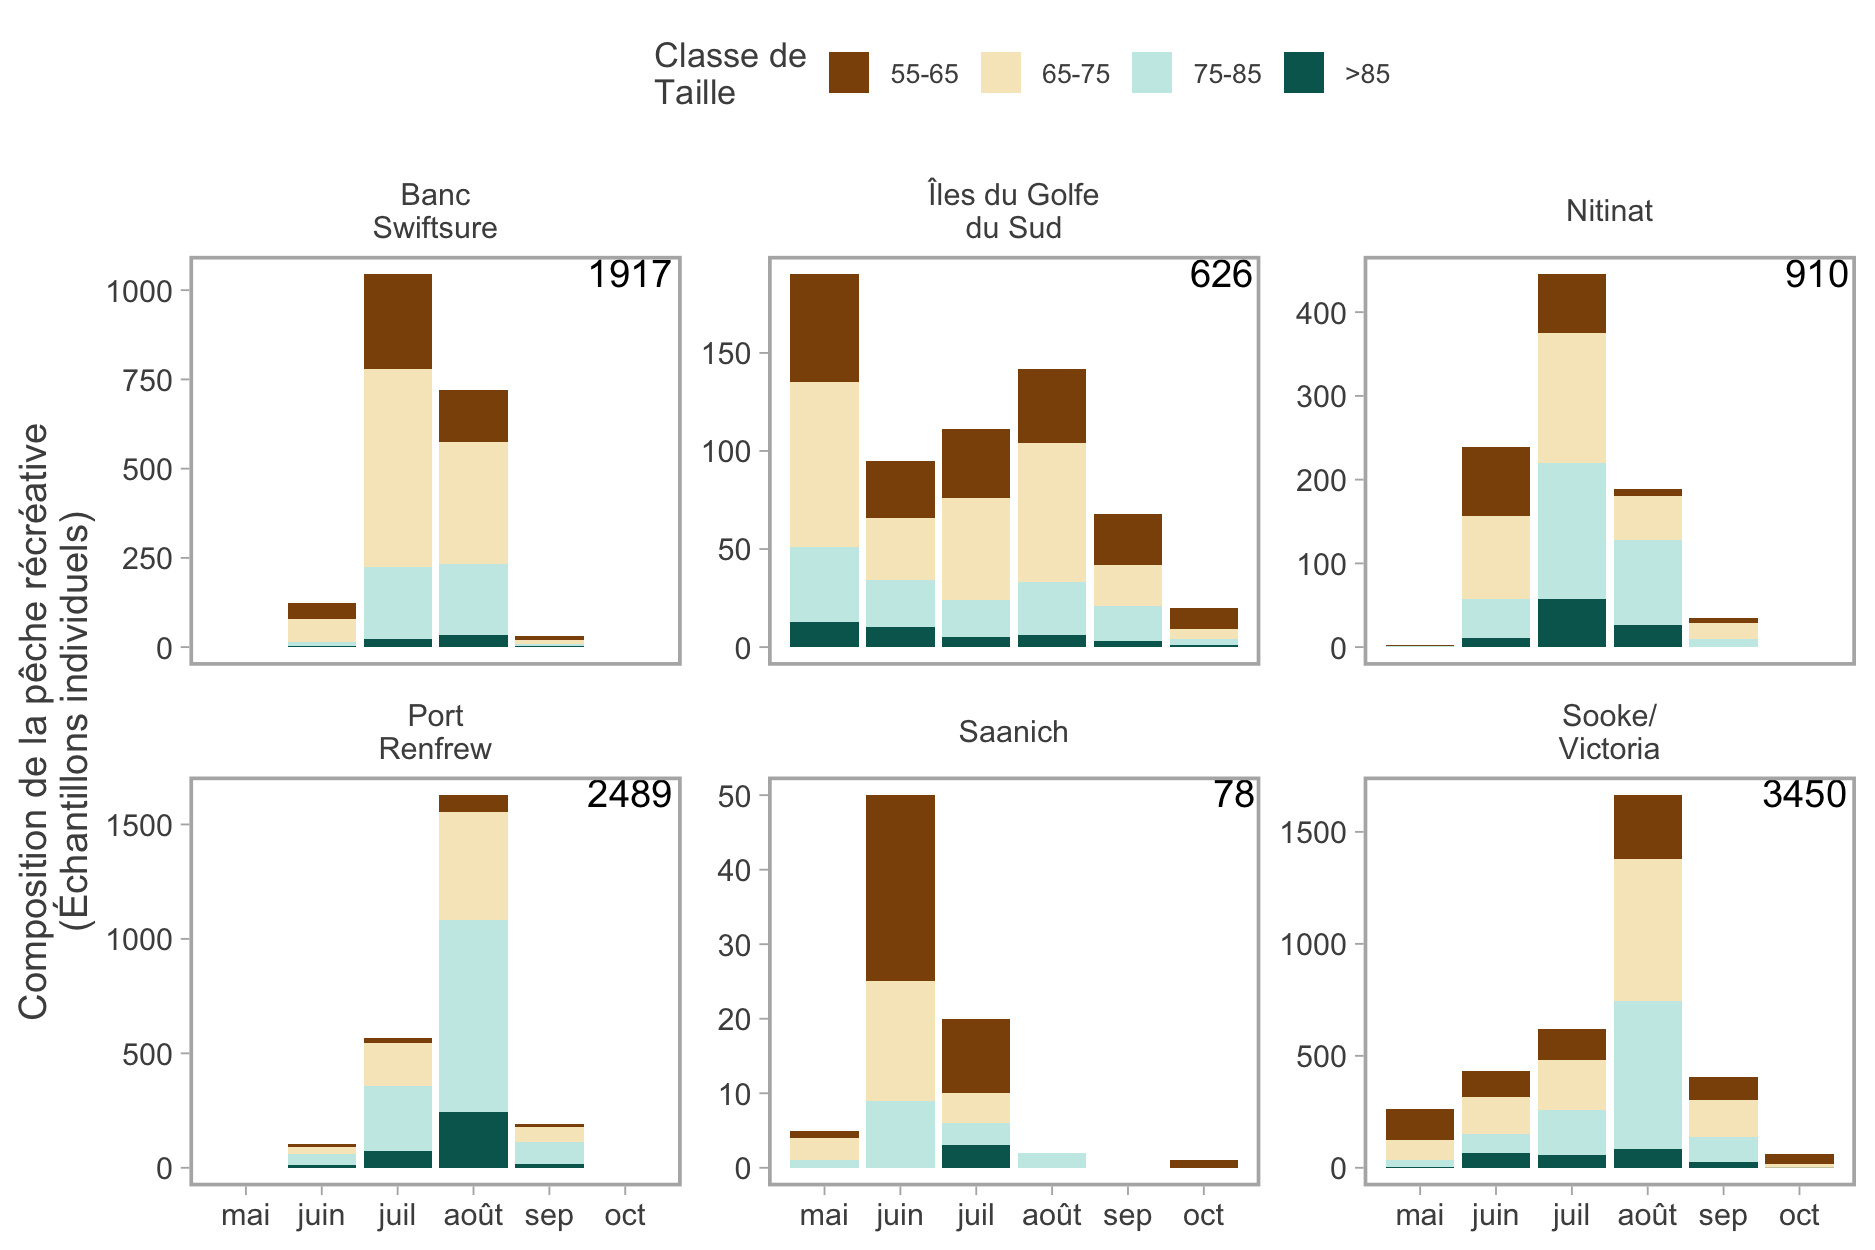
\includegraphics[width=5in]{figs/rec_monthly_size_bar_summer.png}}{Figure \ref{fig:bar-rec-summer-size}}
    \caption{Composition mensuelle de la taille d'échantillons de pêche récréative de saumon quinnat durant les mois d'été. Les strates (panneaux) correspondent aux domaines spatiaux de la Figure \ref{fig:sampling-map}. L'axe des Y représente le nombre d'échantillons collectés dans un mois et une strate spatiale donnés (notez que l'échelle diffère parmi les strates). Les chiffres dans le coin supérieur droit de chaque panneau représentent la taille totale de l'échantillon dans chaque strate.}
    \label{fig:bar-rec-summer-size}
\end{figure}

Les classes de taille du saumon quinnat différaient dans l'abondance moyenne et saisonnière (Figure \ref{fig:season-pred-size}). L'abondance relative de la classe de taille 55-65 cm a décliné à travers l'été avant d'augmenter en septembre, tandis que les individus de 75-85 cm étaient les plus abondants à la fin juillet et en août. Les classes de taille 65-75 cm et supérieure à 85 cm étaient relativement plus stables, bien que les deux aient décliné en septembre (Figure \ref{fig:season-pred-size}).

\begin{figure}[H]
    \centering
    \pdftooltip{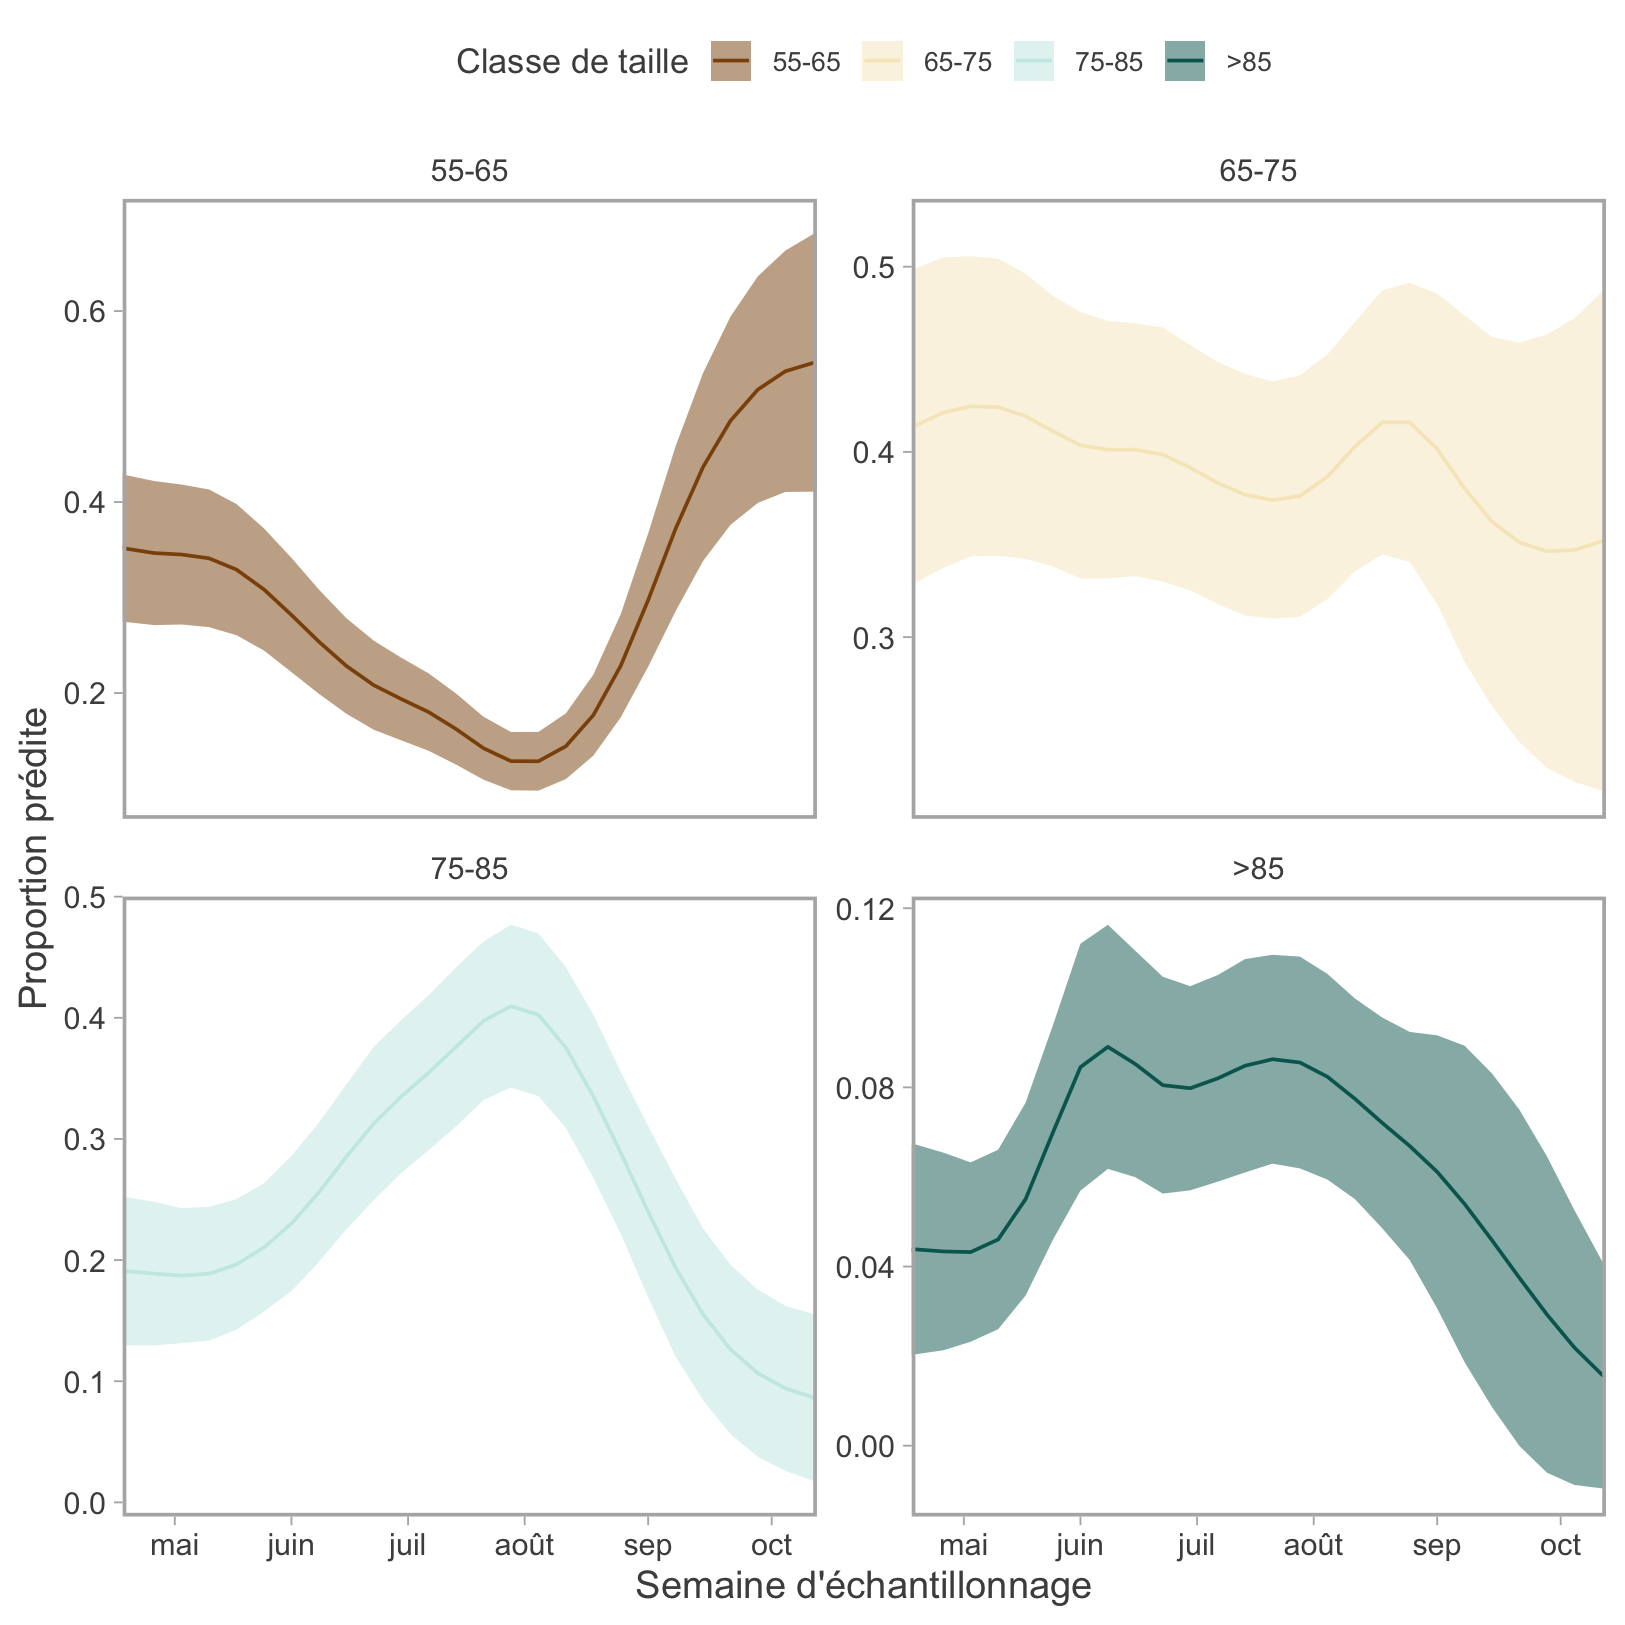
\includegraphics[width=5in]{figs/size_season_preds_chinook.png}}{Figure \ref{fig:season-pred-size}}
    \caption{Composition saisonnière moyenne prédite de la taille basée sur les échantillons de pêche récréative. Le ruban représente l'intervalle de confiance à 95\% de la prédiction moyenne. Les prédictions représentent les effets conditionnels, excluant les termes spatiaux (c.-à-d., représentent l'effet saisonnier « moyen » dans la zone d'étude). Notez que l'échelle de l'axe des y diffère parmi les classes de taille.}
    \label{fig:season-pred-size}
\end{figure}

Les classes de taille du saumon quinnat montraient différentes distributions spatiales entre mai et octobre. La classe de taille 55-65 cm atteignait l'abondance relative maximale près de Victoria et du banc Swiftsure, tandis que l'abondance relative des deux plus grandes classes de taille atteignait un pic près des côtes du banc Swiftsure, ainsi qu'entre Port Renfrew et Sooke. La classe de taille 65-75 cm était plus homogènement distribuée à travers la zone d'étude (Figure \ref{fig:size-spatial-pred-scaled}). La composition de la taille transitait d'être dominée par la classe de taille 65-75 cm au large et sur le banc Swiftsure, vers la classe de taille 75-85 cm près de Port Renfrew, et la plus petite classe de taille au sud de Victoria (Figure \ref{fig:size-spatial-pred}).

\begin{figure}[H]
    \centering
    \pdftooltip{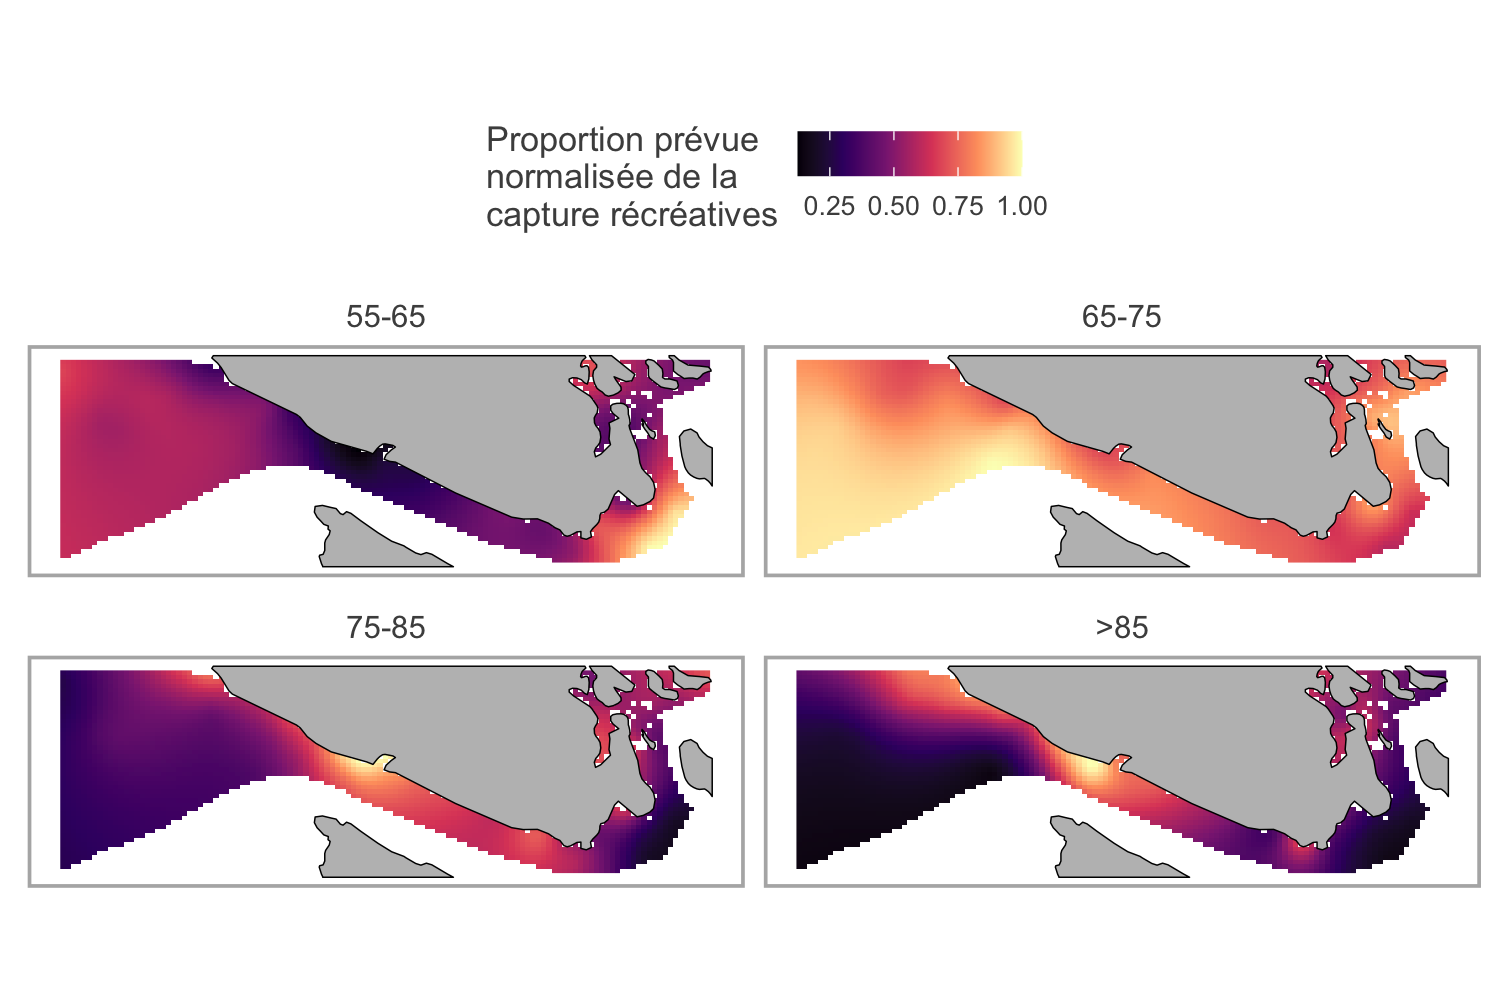
\includegraphics[width=5in]{figs/size_spatial_preds_scaled.png}}{Figure \ref{fig:size-spatial-pred-scaled}}
    \caption{Variation spatiale dans la composition moyenne prédite de la taille mise à l'échelle à travers la portion canadienne du détroit Juan de Fuca et le sud du détroit de Georgie basée sur les échantillons de pêche récréative. Les prédictions sont des moyennes spécifiques aux classes de taille pour mai à octobre et ont été mises à l'échelle relativement à la prédiction maximale à l'intérieur d'une classe de taille pour souligner les différences spécifiques à la taille. Une valeur de un (zéro) indique l'emplacement où une classe de taille était à son abondance prédite maximale (minimale).}
    \label{fig:size-spatial-pred-scaled}
\end{figure}

\begin{figure}[H]
    \centering
    \pdftooltip{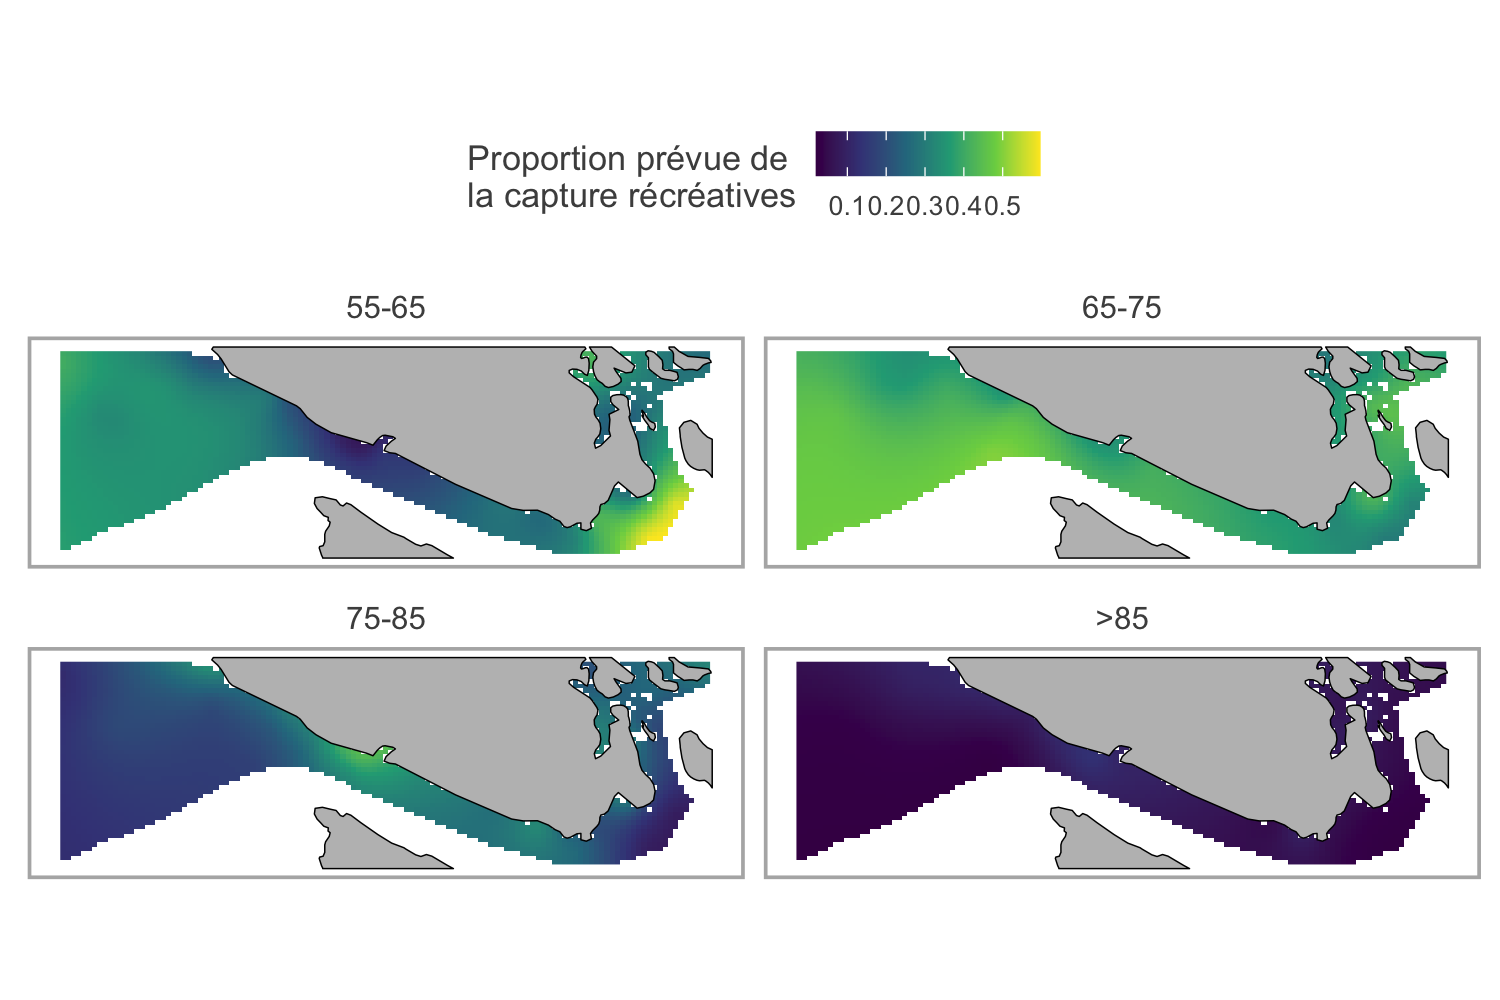
\includegraphics[width=5in]{figs/size_spatial_preds.png}}{Figure \ref{fig:size-spatial-pred}}
    \caption{Variation spatiale dans la composition moyenne prédite de la taille à travers la portion canadienne du détroit Juan de Fuca et le sud du détroit de Georgie basée sur les échantillons de pêche récréative. Les prédictions sont des moyennes spécifiques aux classes de taille pour mai à octobre. Une valeur de un (zéro) indique qu'une classe de taille représentait 100\% (0\%) de l'échantillon moyen prédit.}
    \label{fig:size-spatial-pred}
\end{figure>

Comme pour la composition des stocks, nous avons utilisé un modèle spatio-temporel pour prédire la composition moyenne de la taille à travers l'été pour chaque strate. Le banc Swiftsure et Nitinat avaient des contributions similaires de la plus petite classe de taille, mais Nitinat avait une abondance relativement plus grande des deux plus grandes classes de taille (Figure \ref{fig:stacked-rec}). Port Renfrew avait la contribution relativement la plus grande des grandes classes de taille, avec la proportion moyenne prédite de poissons de plus de 75 cm excédant 65\% en août. Plus à l'est, Sooke/Victoria et les îles Gulf du sud avaient des patrons saisonniers dans la composition de la taille similaires à Nitinat, bien que les poissons plus petits que 55 cm étaient particulièrement abondants à Sooke/Victoria.

\begin{figure}[H]
    \centering
    \pdftooltip{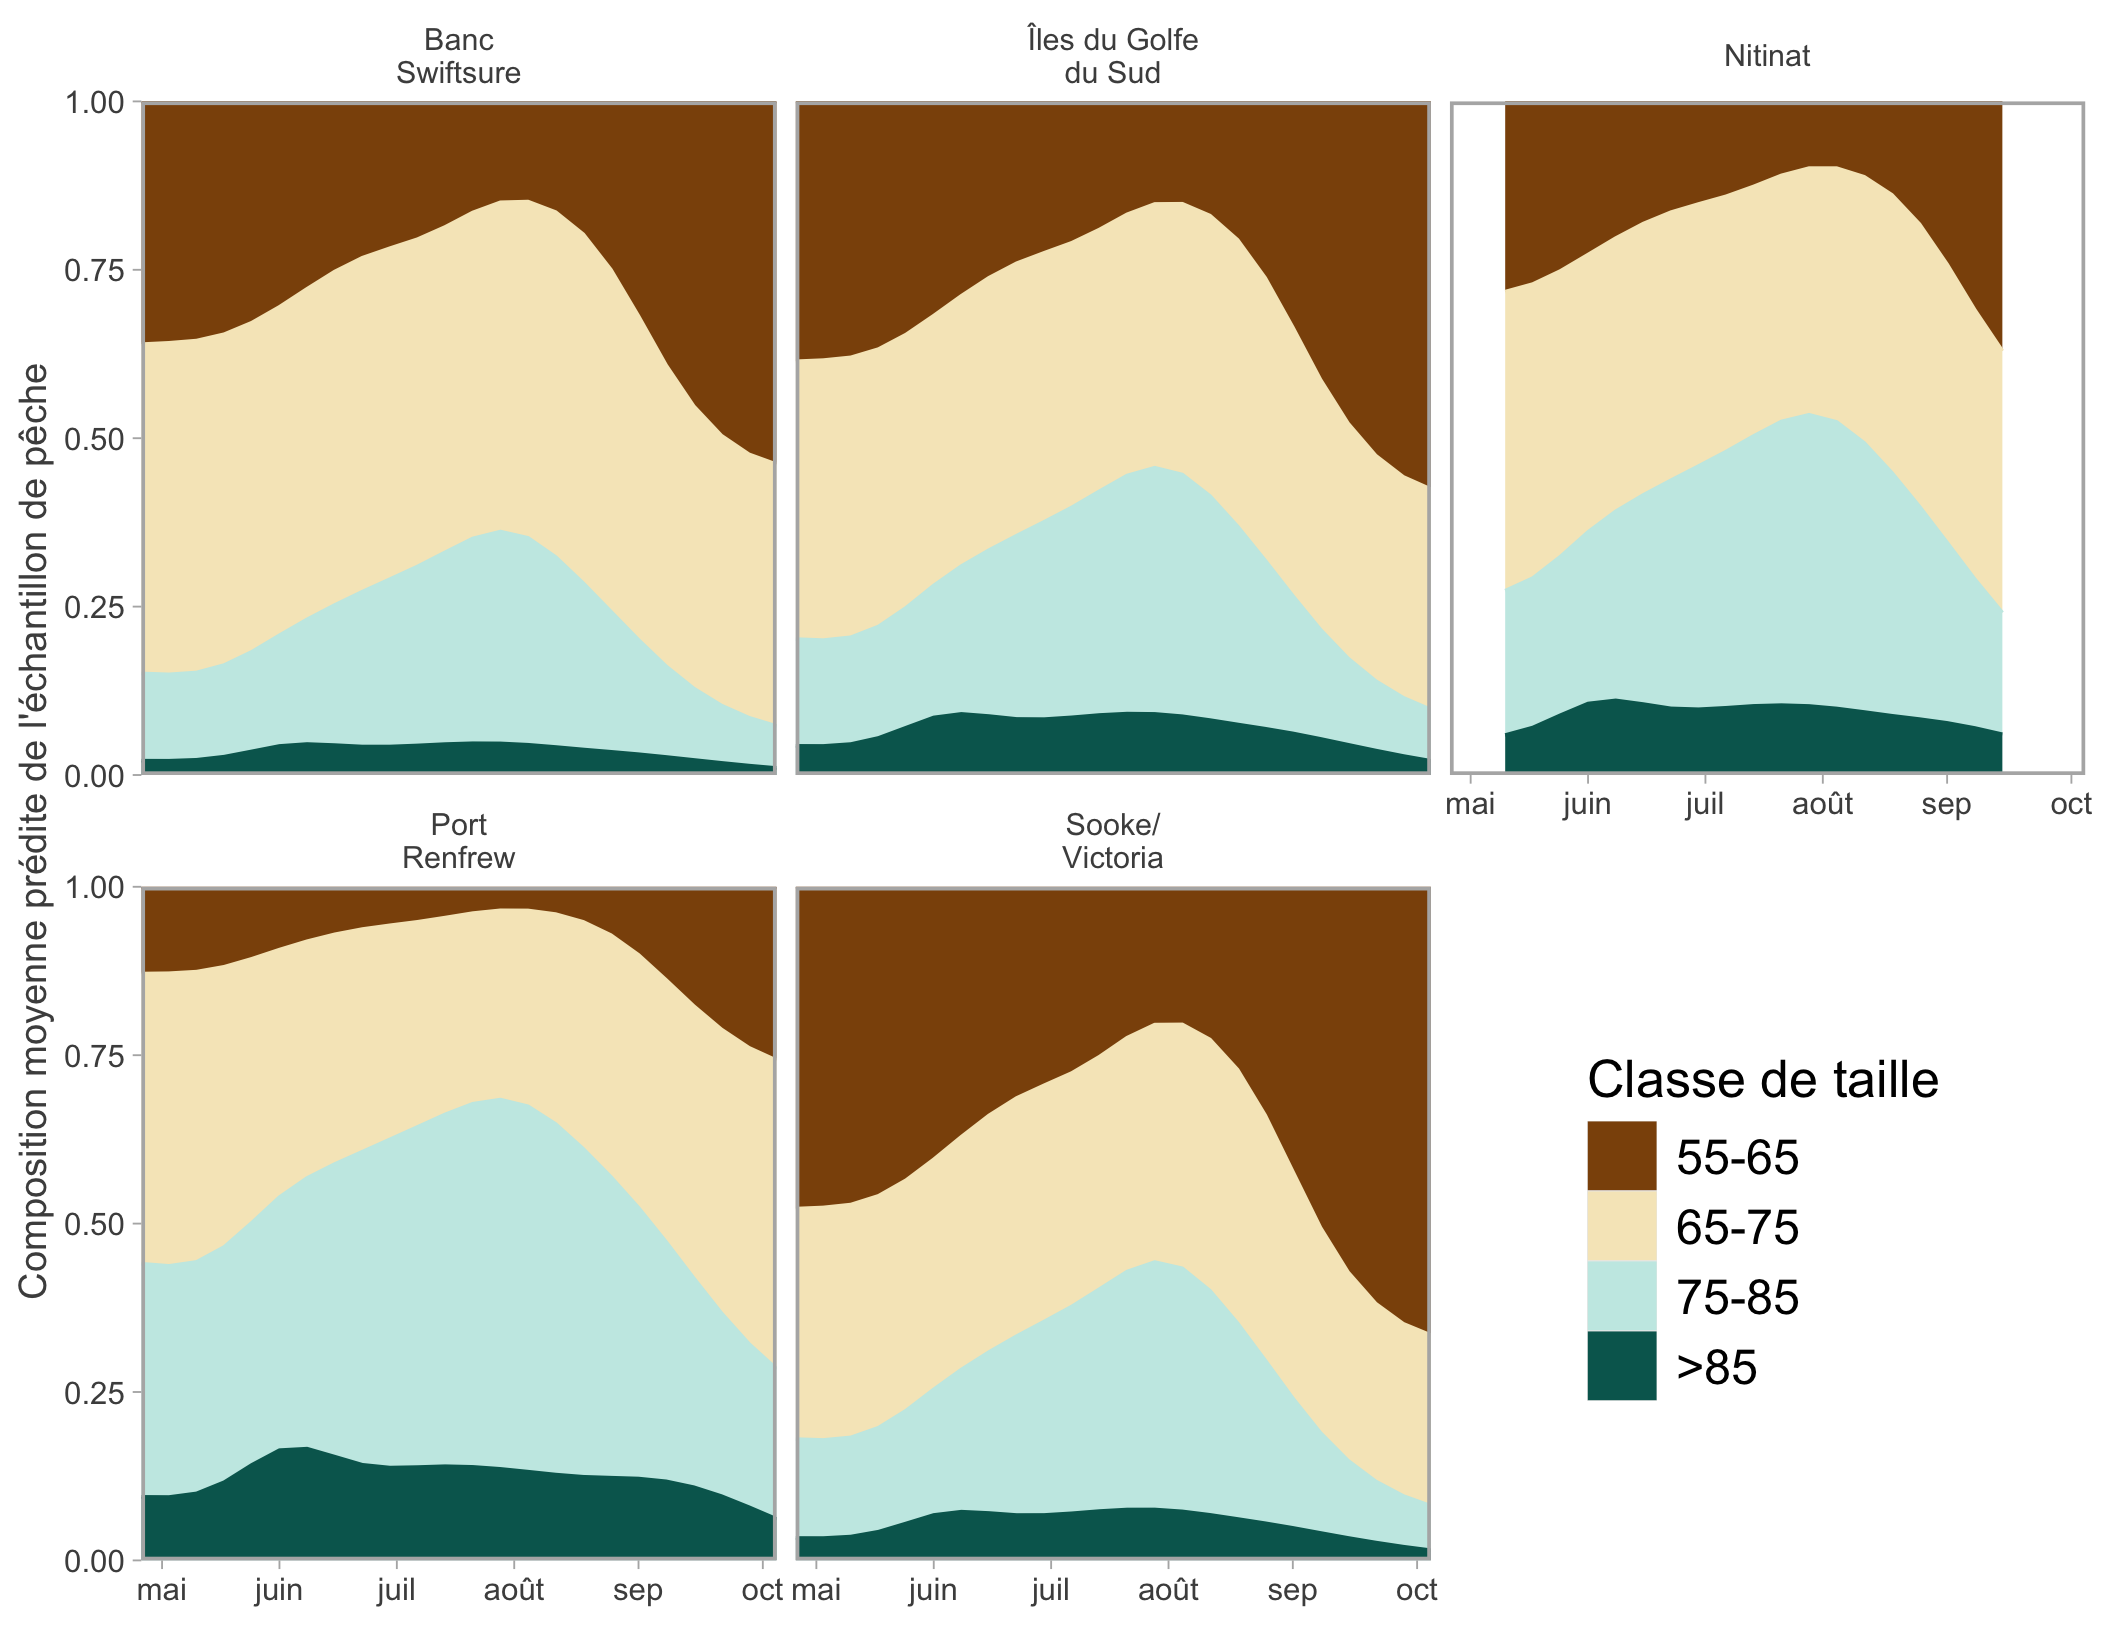
\includegraphics[width=5in]{figs/size_smooth_preds_chinook_stacked.png}}{Figure \ref{fig:stacked-rec-size}}
    \caption{Composition saisonnière moyenne prédite de la taille durant les mois d'été parmi cinq strates spatiales basée sur les échantillons de pêche récréative. Les prédictions ont été estimées en utilisant les emplacements (représentés par un « x ») à l'intérieur de chaque domaine spatial de la Figure \ref{fig:sampling-map} et excluent la variabilité interannuelle. Saanich non montré en raison de données limitées en juillet et août, ainsi que son emplacement à l'extérieur de l'habitat essentiel des ÉRES.}
    \label{fig:stacked-rec-size}
\end{figure}

L'abondance relative de différentes classes de taille variait considérablement parmi les années (Figure \ref{fig:size-smooth-pred-rec-year}). Par exemple, la proportion moyenne prédite de l'échantillon appartenant à la classe de taille supérieure à 85 cm à Port Renfrew en juin variait de 7,7\% à 20,9\% parmi les années d'échantillonnage.

Les résidus du modèle de composition de la taille ajusté étaient appropriément distribués (Figure \ref{fig:qqplot-size}) et les vérifications prédictives postérieures ont confirmé que la composition moyenne simulée des stocks, tenant compte de la variance résiduelle, était généralement similaire à la composition observée de la taille (Figure \ref{fig:posterior-size}). Comme pour le modèle de composition des stocks, les déviations les plus fortes étaient dans les strates avec relativement peu d'échantillons (p. ex., Saanich) ou les classes de taille et strates avec des patrons saisonniers fortement non-linéaires (p. ex., 55-65 cm dans les îles Gulf du sud).

\subsubsection{Contribution des écloseries}

De mai à octobre, le statut d'origine d'écloserie ou sauvage pouvait être déterminé pour la plupart des échantillons de la pêche récréative. Les individus d'origine d'écloserie étaient relativement communs dans toutes les strates, mais constituaient la majorité de la capture dans la plupart des mois dans les strates du banc Swiftsure, Nitinat, et Saanich (Figure \ref{fig:bar-hatchery-summer}). Inversement, les poissons d'origine sauvage étaient relativement plus abondants, particulièrement en août, dans les strates Port Renfrew et Sooke/Victoria (Figure \ref{fig:bar-hatchery-summer}).

\begin{figure}[H]
    \centering
    \pdftooltip{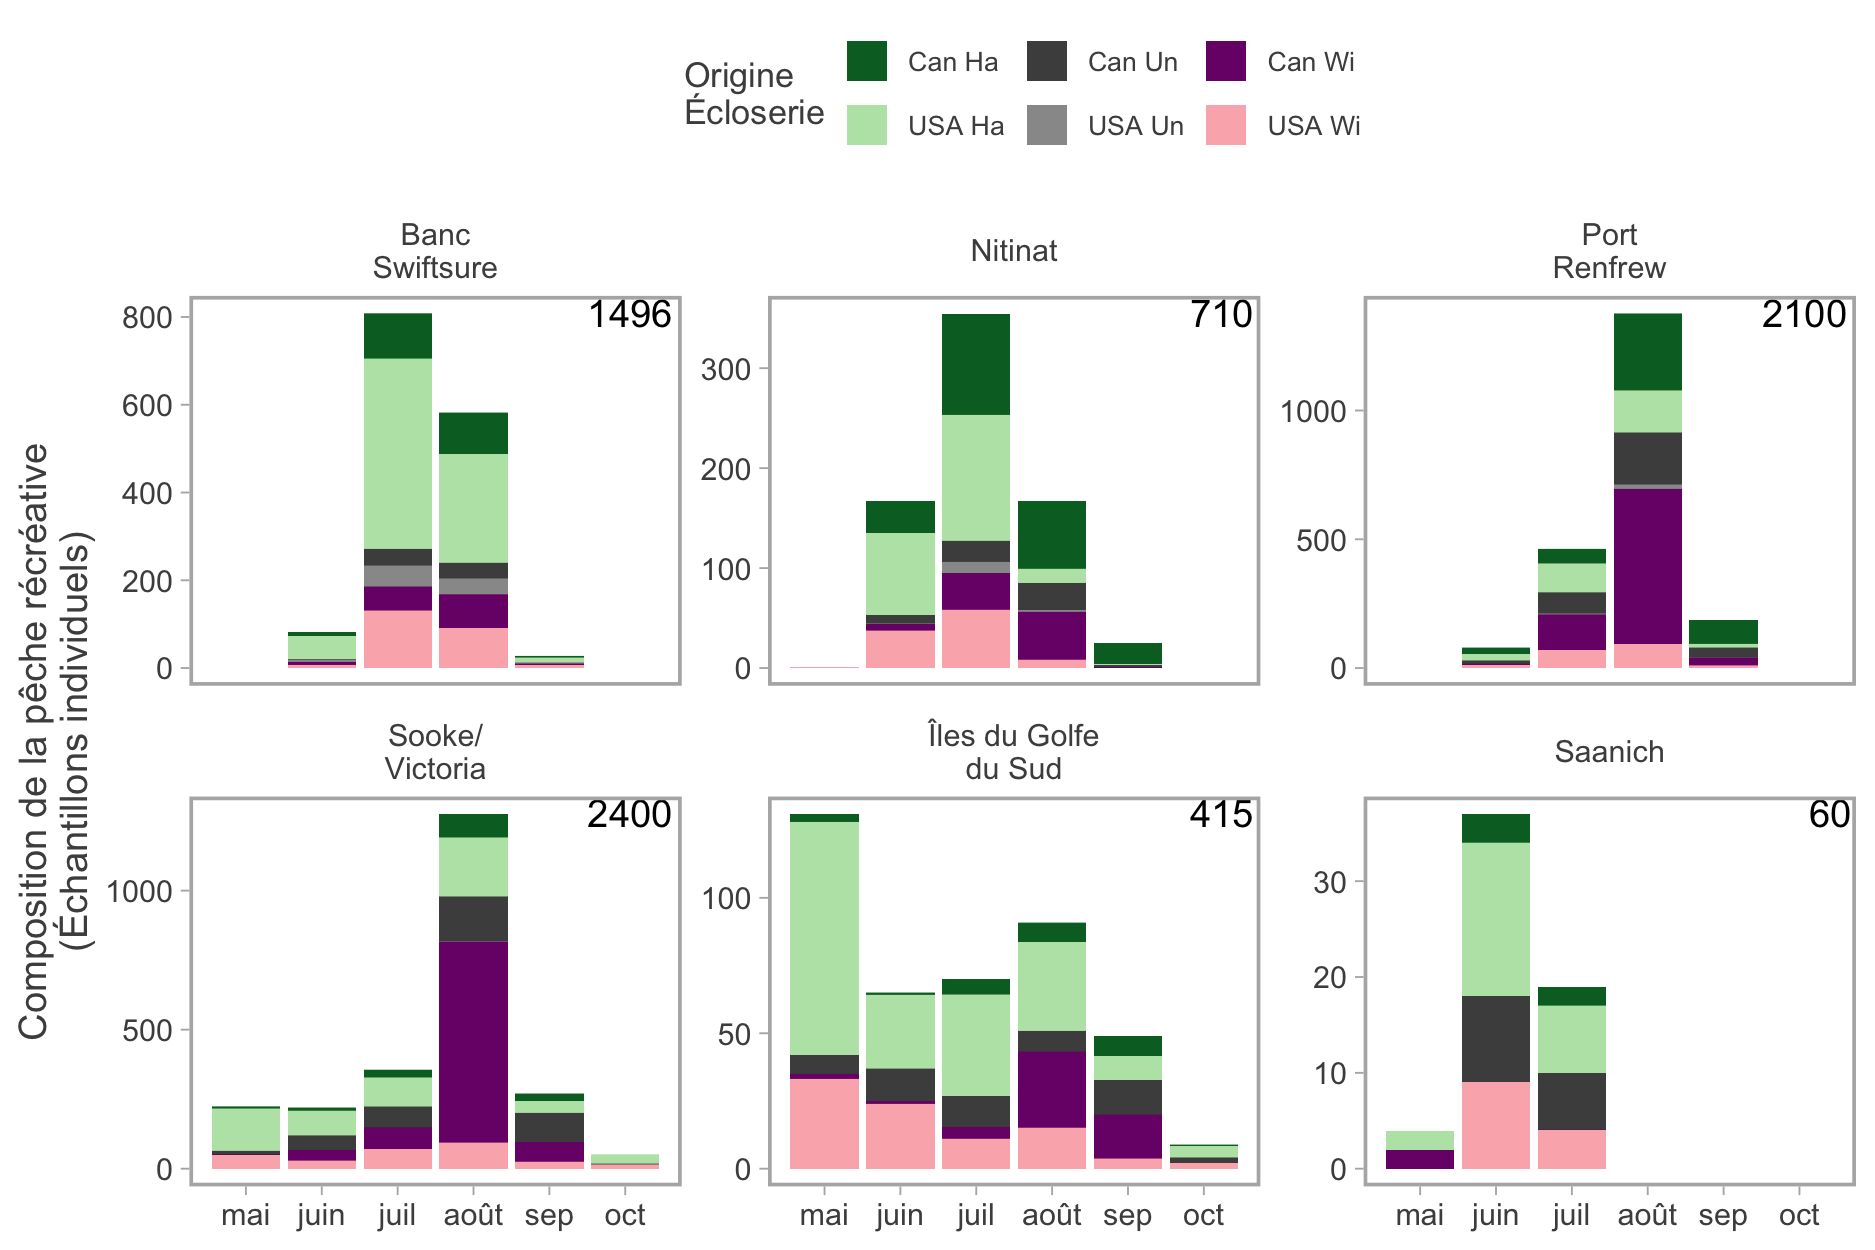
\includegraphics[width=5in]{figs/rec_monthly_hatchery_comp_bar_summer.png}}{Figure \ref{fig:bar-hatchery-summer}}
    \caption{Abondance relative d'individus d'origine d'écloserie (vert), sauvage (violet), et inconnue (gris), groupés par pays (Canada foncé; États-Unis pâle). Les assignations inconnues se sont produites quand un individu avec une nageoire adipeuse intacte était assigné, basé sur l'ISG, à un stock sans marquage de masse et couverture de marquage basé sur la parenté incomplète.}
    \label{fig:bar-hatchery-summer}
\end{figure}

Les stocks différaient dans la contribution relative d'individus d'origine d'écloserie, sauvage et inconnue. La majorité des individus des stocks américains étaient d'origine d'écloserie (approximativement 55-75\%) et relativement peu étaient non assignés en raison de la prévalence du marquage de masse dans les écloseries de Washington et de l'Oregon (Figure \ref{fig:bar-hatchery-stocks}). La contribution de poissons d'écloserie aux stocks canadiens était plus variable et il y avait une plus grande proportion d'individus d'origine inconnue due au fait que peu d'écloseries canadiennes emploient le marquage de masse. Bien que la couverture TPB soit actuellement répandue dans les écloseries canadiennes, la couverture a varié à travers le temps et était faible avant l'année de ponte 2013 (Figure \ref{fig:pbt-coverage}). Ainsi plusieurs poissons, particulièrement ceux capturés avant approximativement 2017, ne pouvaient pas être assignés un statut d'écloserie de manière fiable.

\begin{figure}[H]
    \centering
    \pdftooltip{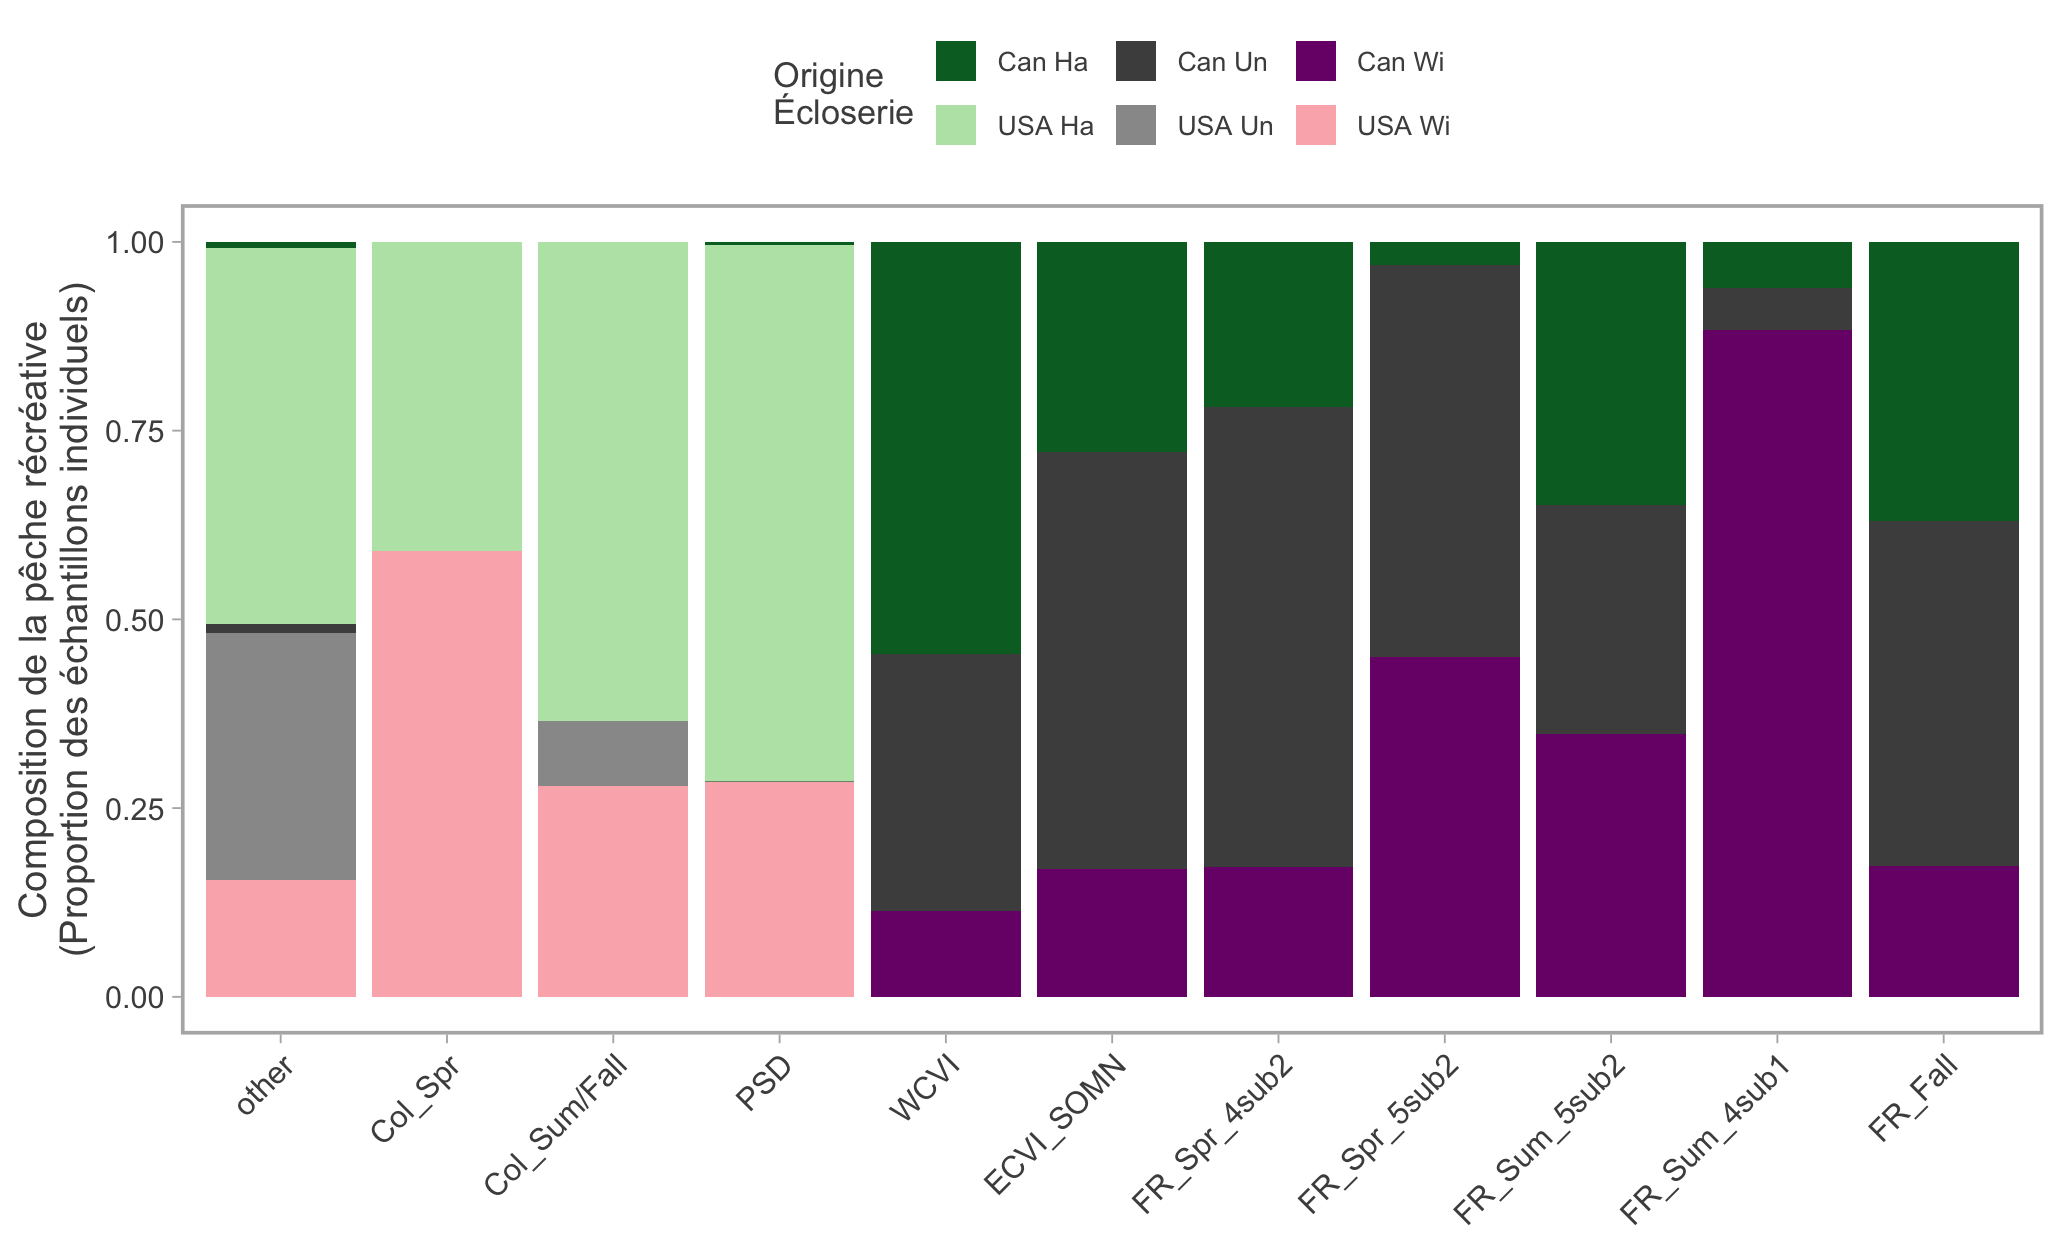
\includegraphics[width=5in]{figs/rec_stock_hatchery_bar.png}}{Figure \ref{fig:bar-hatchery-stocks}}
    \caption{Abondance relative d'individus d'origine d'écloserie (vert), sauvage (violet), et inconnue (gris) dans chaque stock. Les assignations inconnues se sont produites quand un individu avec une nageoire adipeuse intacte était assigné à un stock sans marquage de masse ou couverture de marquage basé sur la parenté incomplète.}
    \label{fig:bar-hatchery-stocks}
\end{figure}

La proportion de géniteurs d'origine d'écloserie (pHOS) entre 2014 et 2022 différait parmi les stocks canadiens et parmi les années (Figure \ref{fig:box-phos}). Le pHOS moyen était de 72\% parmi les populations surveillées dans le stock COIV et de 53\% pour les populations à l'intérieur du stock COIV/SOMN. Les niveaux pHOS étaient légèrement plus bas parmi les stocks de la rivière Fraser, mais la plupart des stocks avaient seulement une ou deux populations améliorées par écloserie (Figure \ref{fig:box-phos}). Il y avait une variabilité considérable parmi les populations à l'intérieur d'un stock, soulignant que les estimations au niveau des stocks des contributions d'écloserie basées sur le pHOS seul devraient être interprétées avec prudence.

\subsection{Sélectivité dans les restes de proies des ÉRES}

Nous avons utilisé des simulations Monte Carlo pour tester l'évidence que la composition observée des stocks et de la taille des restes de proies des ÉRES (collectés après 2016 et dans les strates du banc Swiftsure, Nitinat, et Port Renfrew) déviait de la composition attendue telle qu'indexée par la pêche récréative. Notre approche tenait compte de la variabilité spatiale, saisonnière, et interannuelle en utilisant les modèles de composition décrits précédemment, tout en propageant l'incertitude due à l'assignation génétique des stocks, l'assignation de l'âge, les petites tailles d'échantillon, et les paramètres estimés du modèle.

Nous avons trouvé de l'évidence de sélection positive pour les stocks Fraser rivière printemps $5.2$, été $5.2$, et été $4.1$ (Figure \ref{fig:sel-stock}). Ces stocks constituaient 4-36\% de plus de l'échantillon observé de restes de proies que prédit par le modèle de composition des stocks paramétrisé avec les données de pêche récréative. Inversement, les stocks COIV, Puget Sound, Columbia été/automne, et « Autre » étaient sous-représentés dans les restes de proies, avec leur contribution proportionnelle 5-27\% de moins que la prédiction du modèle (Figure \ref{fig:sel-stock}). Il n'y avait pas d'évidence de sélectivité dans les stocks restants, probablement parce que leur abondance relative observée était faible dans les restes de proies et prédite pour être faible aux moments et emplacements où les restes de proies ont été collectés (Figures \ref{fig:bar-diet}, \ref{fig:stacked-rec}).

\begin{figure}[H]
    \centering
    \pdftooltip{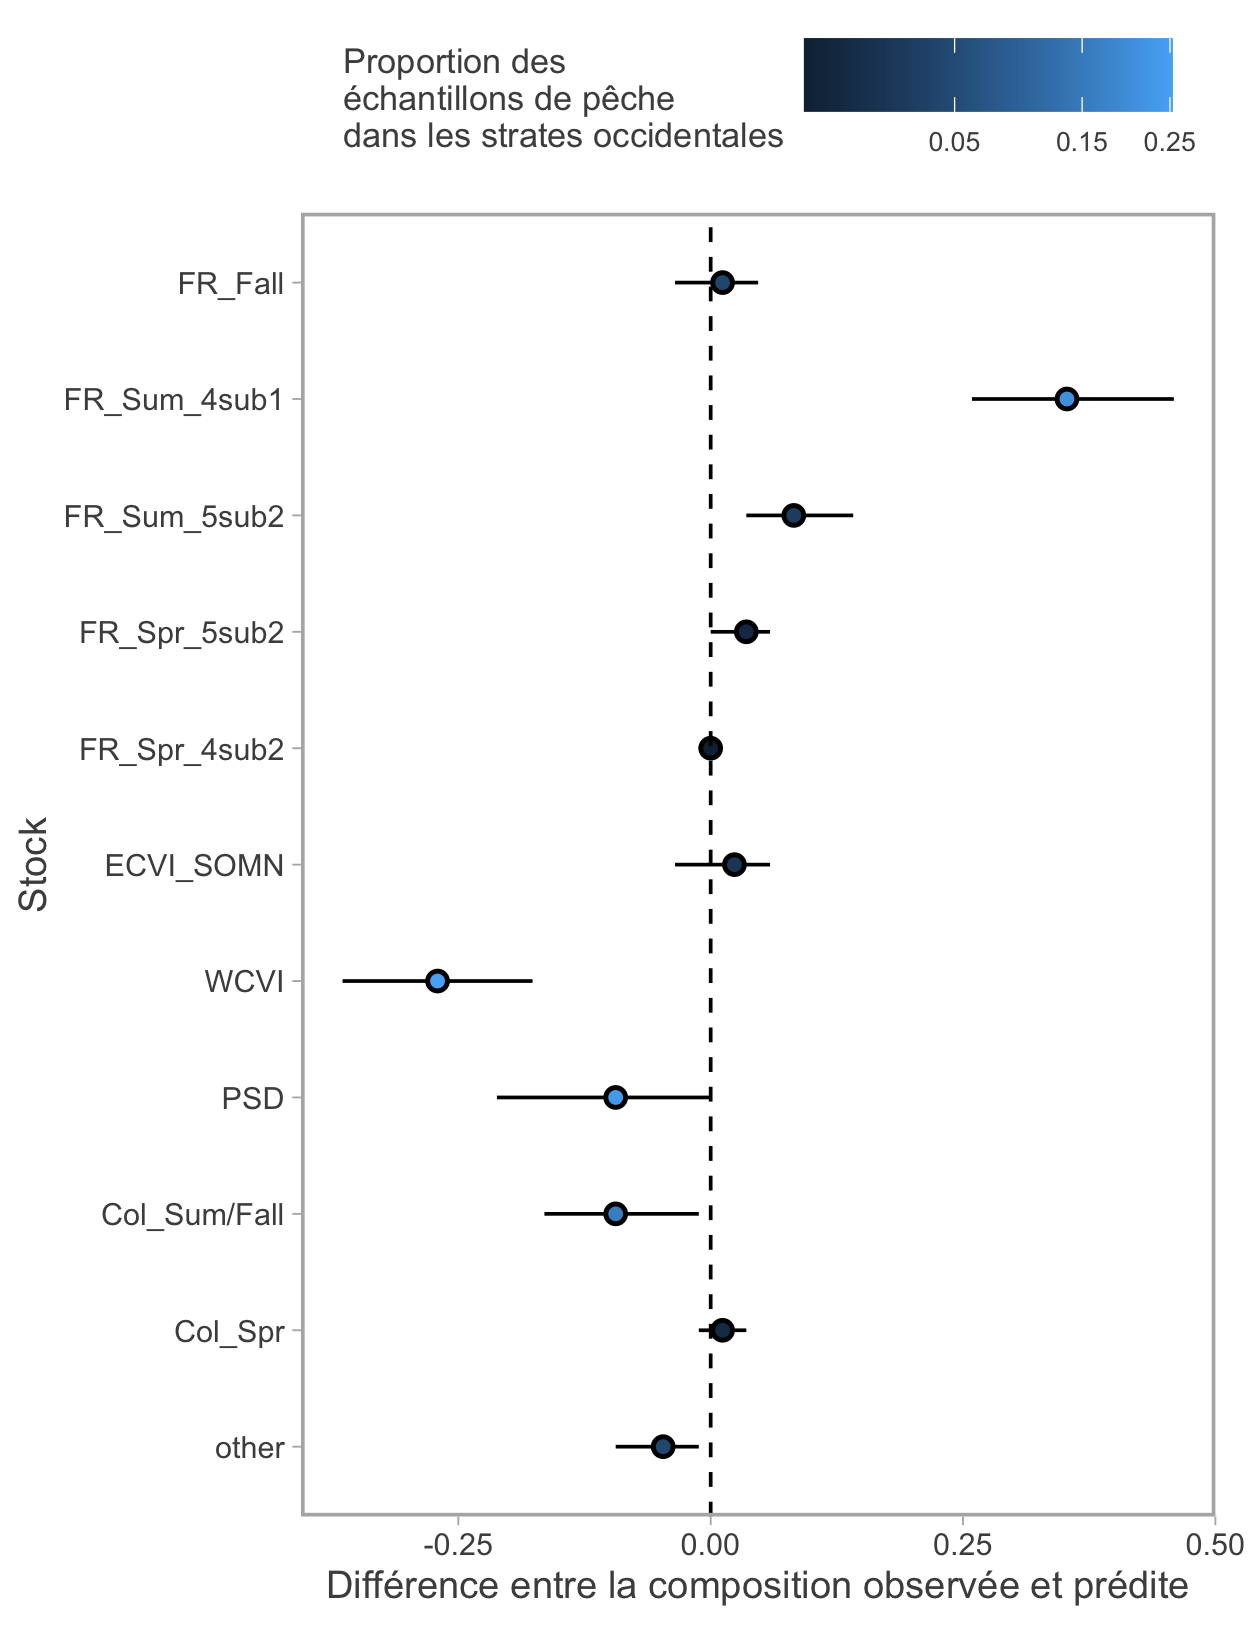
\includegraphics[width=5in]{figs/selectivity_bean_stock.png}}{Figure \ref{fig:sel-stock}}
    \caption{Différences entre la contribution observée et prédite par le modèle de chaque stock aux restes de proies des ÉRES. Les valeurs positives (négatives) indiquent qu'un stock donné était observé plus (moins) fréquemment dans les restes de proies des ÉRES que prédit par le modèle dépendant de la pêche. Les points représentent les médianes et les moustaches représentent les intervalles du 95e percentile parmi 500 simulations Monte Carlo. Les points plus brillants (plus foncés) représentent les stocks qui étaient plus (moins) communs dans les échantillons de pêche récréative des moments et strates coïncidents avec les restes de proies des ÉRES.}
    \label{fig:sel-stock}
\end{figure}

Les deux plus petites classes de taille du saumon quinnat constituaient une proportion plus petite (approximativement 10\% et 7\% respectivement) des restes de proies observés que prédit par le modèle de composition de la taille paramétrisé avec les données de pêche récréative (Figure \ref{fig:sel-size}). Nous avons aussi trouvé de l'évidence de sélection positive pour les deux plus grandes classes de taille, qui étaient approximativement 8\% plus communes dans les restes de proies observés que prédit par le modèle (Figure \ref{fig:sel-size}). Les estimations de sélectivité pour les deux classes de taille intermédiaires (65-75 et 75-85 cm) étaient plus incertaines que les deux autres classes de taille malgré des médianes similaires (Figure \ref{fig:sel-size}).

\begin{figure}[H]
    \centering
    \pdftooltip{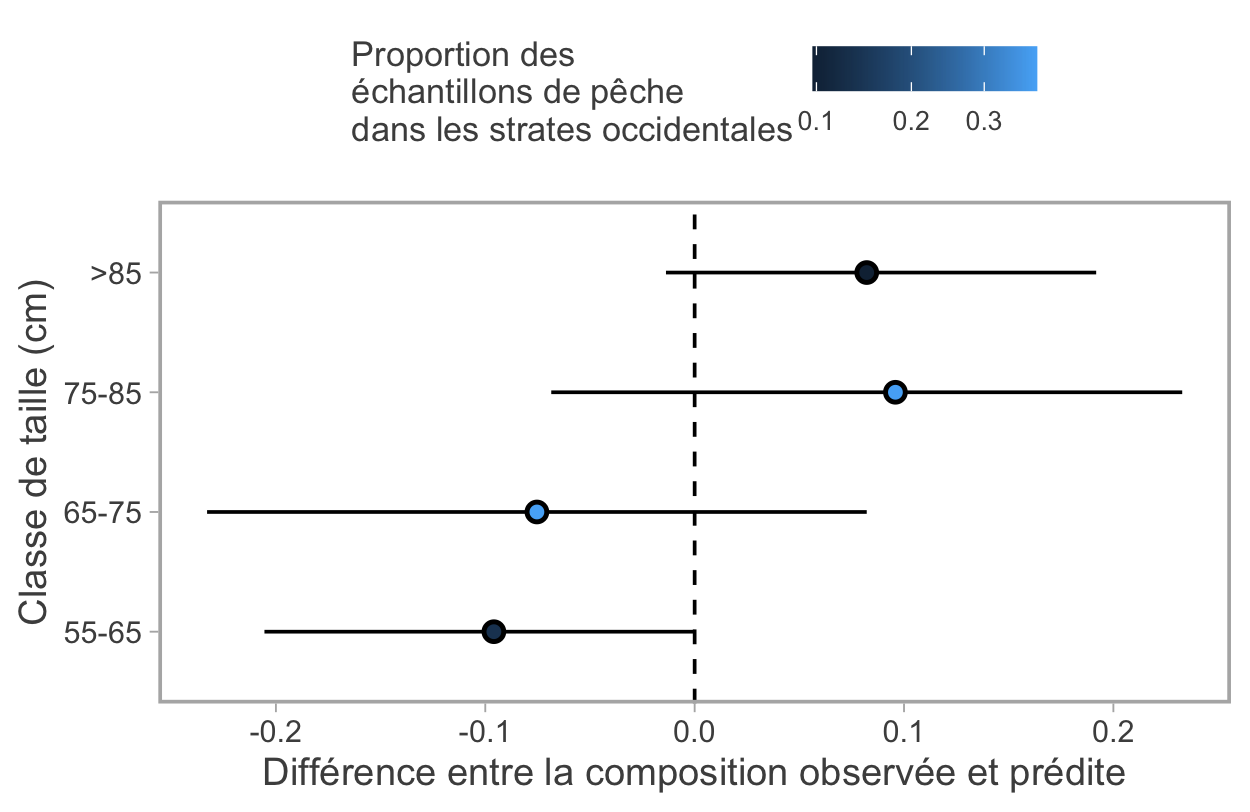
\includegraphics[width=5in]{figs/selectivity_bean_size.png}}{Figure \ref{fig:sel-size}}
    \caption{Différences entre la contribution observée et prédite par le modèle de chaque classe de taille aux restes de proies des ÉRES. Les valeurs positives (négatives) indiquent qu'une classe de taille donnée était observée plus (moins) fréquemment dans les restes de proies des ÉRES que prédit par le modèle dépendant de la pêche. Les points représentent les médianes et les moustaches représentent les intervalles du 95e percentile parmi 500 simulations Monte Carlo. Les points plus brillants (plus foncés) représentent les classes de taille qui étaient plus (moins) communes dans les échantillons de pêche récréative des moments et strates coïncidents avec les restes de proies des ÉRES.}
    \label{fig:sel-size}
\end{figure>

\subsection{Analyses de sensibilité}

Le modèle de composition des stocks qui a été ajusté aux données qui incluaient seulement les échantillons de pêches récréatives supérieurs à 75 cm de longueur à la fourche a prédit une composition des stocks légèrement différente, particulièrement tôt dans l'année (Figures \ref{fig:comb-pred-stock1}, \ref{fig:comb-pred-stock2}). Cependant, les mêmes stocks montraient de l'évidence de sélectivité positive et négative (Figure \ref{fig:comb-sel-stock}). Similairement, les résultats de sélectivité des stocks et de sélectivité de la taille étaient similaires quand les échantillons qui chevauchaient avec les interventions de gestion des pêches étaient exclus. Détails additionnels dans l'Annexe \ref{sensitivity}.

\subsection{Abondance terminale du saumon quinnat}

Tous les stocks de saumon quinnat présents dans la zone d'étude ont montré des tendances cycliques dans l'abondance terminale au cours des 40 dernières années; cependant, ces dynamiques n'ont pas été homogènes. Les stocks côtiers de Washington et de l'Oregon (inclus dans le stock « Autre » à travers cette analyse); Columbia rivière printemps; et Fraser rivière printemps $4_2$, printemps $5_2$, et été $5_2$ ont décliné à travers les années 2010 et ont montré des degrés variables de récupération (Figure \ref{fig:esc-stock}). Inversement, l'abondance terminale des stocks COIV, COIV/SOMN, et Fraser rivière été $4_1$ a augmenté (Figure \ref{fig:esc-stock}).

\begin{figure}[H]
    \centering
    \pdftooltip{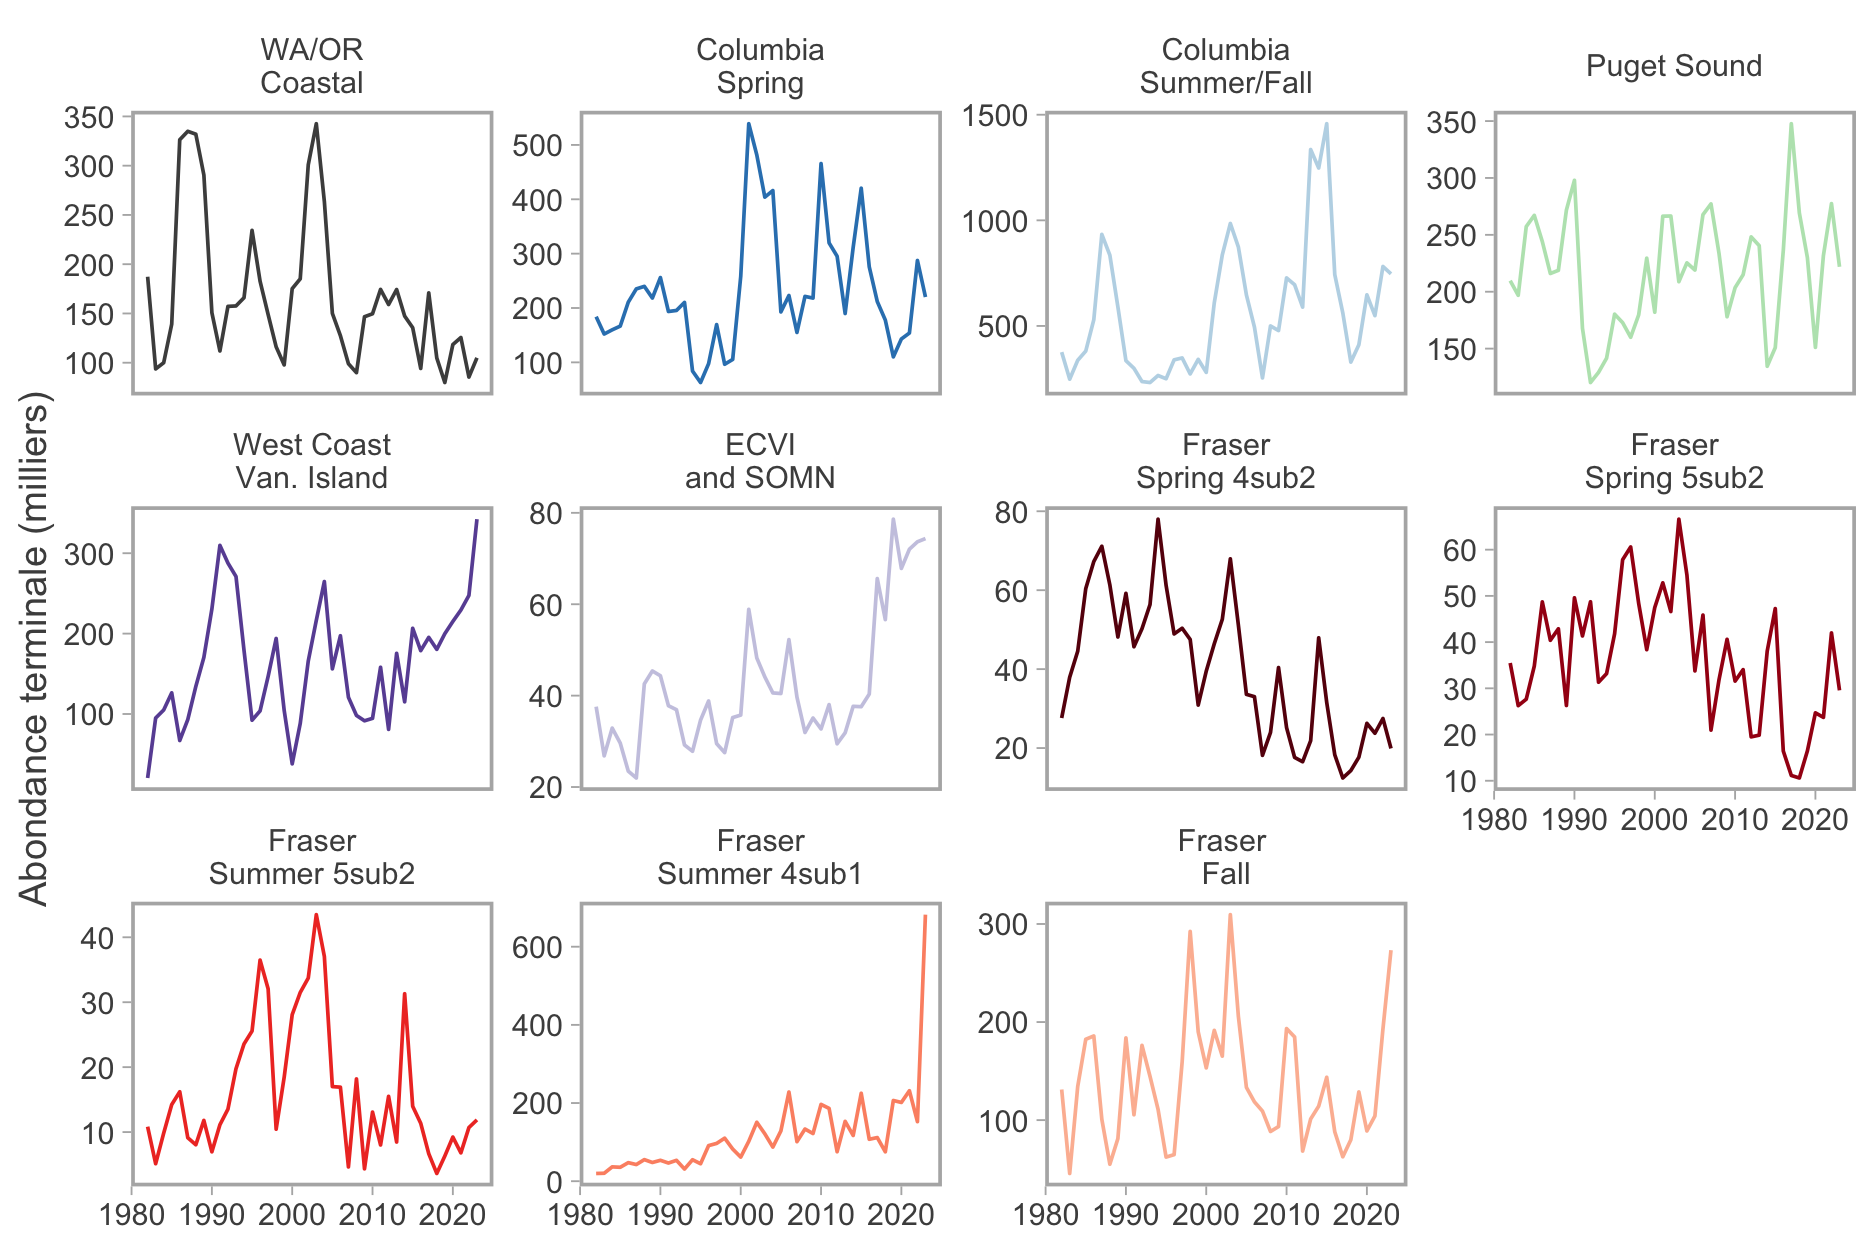
\includegraphics[width=5in]{figs/escapement_stock_group.png}}{Figure \ref{fig:esc-stock}}
    \caption{Abondance terminale des stocks de saumon quinnat. Les populations côtières de Washington et de l'Oregon (WA/OR) sont incluses dans le stock « Autre » à travers ce manuscrit. Les données de 2023 n'étaient pas disponibles pour les stocks côtiers WA/OR et Puget Sound et ont été imputées basées sur les moyennes 2019-2022. Les échelles de l'axe des Y diffèrent parmi les stocks. Définitions de l'abondance terminale et sources de données disponibles dans l'Annexe \ref{terminal-abundance}.}
    \label{fig:esc-stock}
\end{figure}

L'abondance terminale agrégée (c.-à-d., sommée parmi les stocks) a aussi varié cycliquement, mais est relativement élevée comparée à l'abondance terminale avant 2000 (Figure \ref{fig:esc-stock}). Généralement la majorité de l'abondance terminale agrégée provient des stocks de la côte extérieure (côtiers de Washington et de l'Oregon, Columbia rivière, côte ouest de l'île de Vancouver); cependant, la contribution des stocks qui frayent dans les bassins versants de la mer des Salish a augmenté durant les années récentes.

\begin{figure}[H]
    \centering
    \pdftooltip{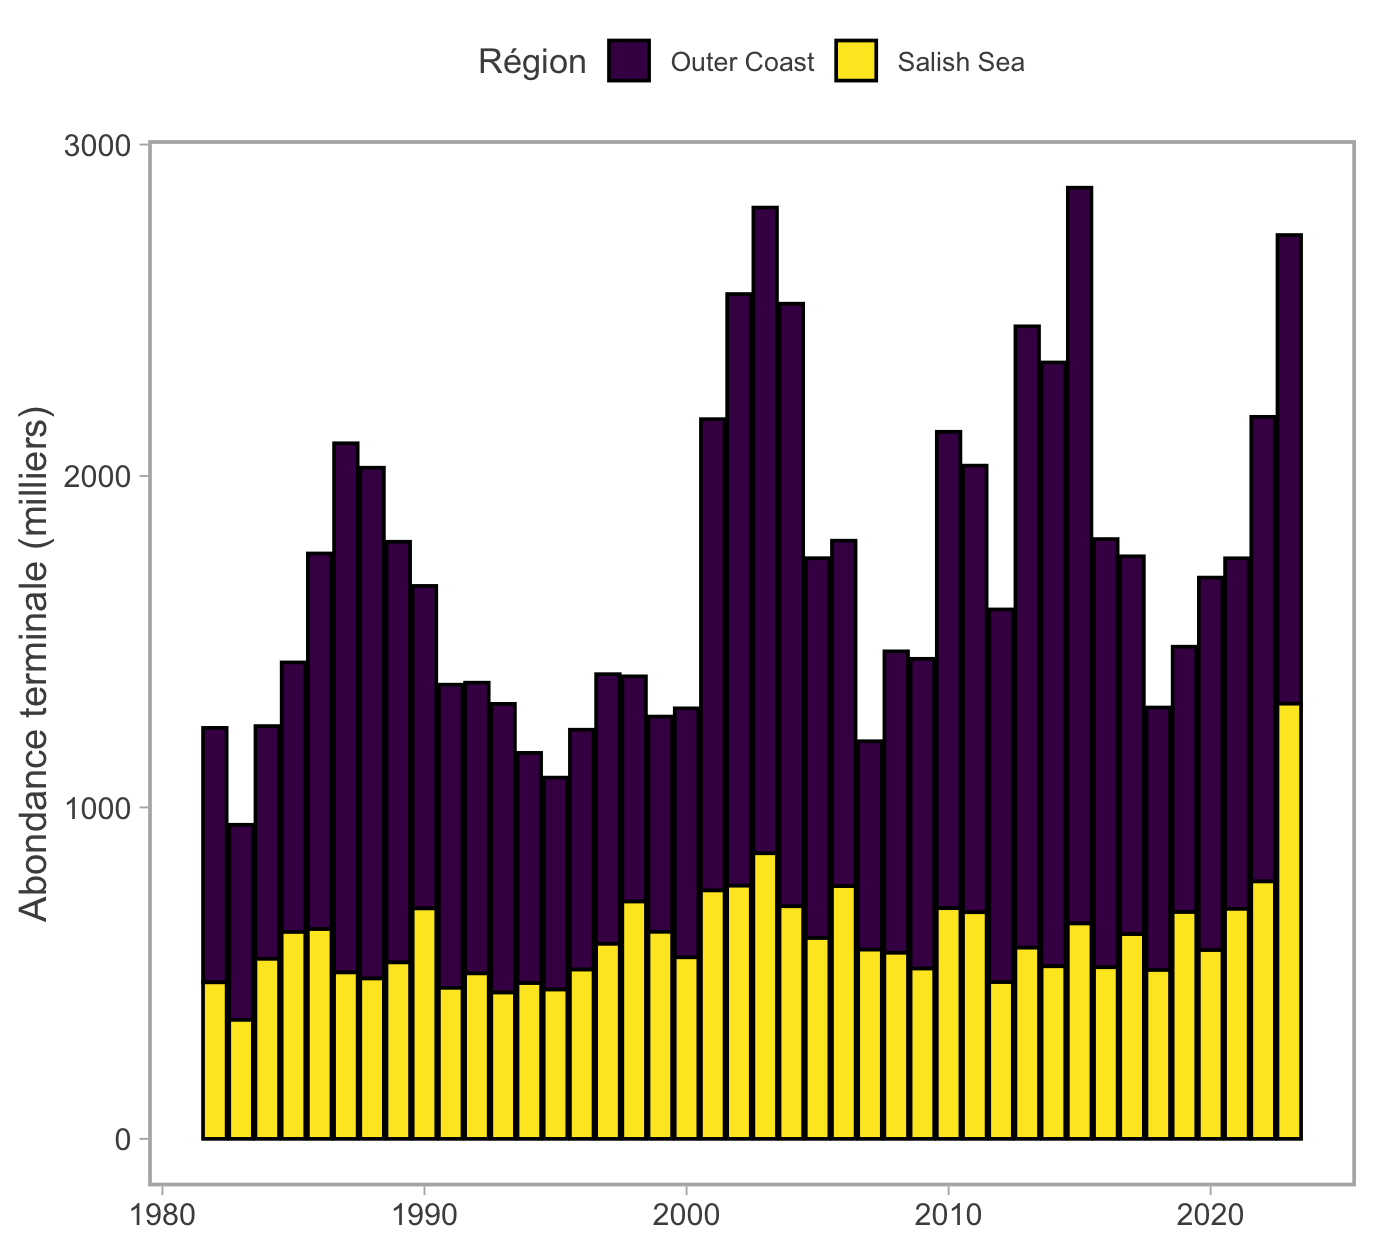
\includegraphics[width=5in]{figs/escapement_region.png}}{Figure \ref{fig:esc-region}}
    \caption{Abondance terminale agrégée des stocks de saumon quinnat, communs dans l'habitat essentiel des ÉRES, frayant à l'intérieur de la mer des Salish (jaune) ou dans la côte extérieure, incluant la Columbia rivière (violet). Les barres légèrement ombrées représentent les valeurs moyennes sur cinq ans. 2023 n'est pas montré étant donné les données manquantes pour les stocks côtiers de Washington et Puget Sound. Définitions de l'abondance terminale et sources de données disponibles dans l'Annexe \ref{terminal-abundance}.}
    \label{fig:esc-region}
\end{figure}